% RDT2 Technical Report - Comprehensive Beamer Presentation
% Theme: Beaver (default)
% Purpose: Understanding RDT2 architecture for ManiSkill debugging

\documentclass[aspectratio=169, 10pt]{beamer}

% Theme
\usetheme{Beaver}
\usecolortheme{beaver}

% Packages
\usepackage[utf8]{inputenc}
\usepackage[T1]{fontenc}
\usepackage{tikz}
\usepackage{pgfplots}
\usepackage{amsmath, amssymb}
\usepackage{booktabs}
\usepackage{listings}
\usepackage{xcolor}
\usepackage{hyperref}
\usepackage{graphicx}
\usepackage{subcaption}
\usepackage{multirow}
\usepackage{array}

% TikZ Libraries
\usetikzlibrary{
    shapes.geometric,
    shapes.arrows,
    arrows.meta,
    positioning,
    calc,
    fit,
    backgrounds,
    decorations.pathreplacing,
    decorations.markings,
    patterns,
    matrix,
    chains,
    scopes
}

% PGFPlots settings
\pgfplotsset{compat=1.18}

% Colors
\definecolor{qwenblue}{RGB}{70, 130, 180}
\definecolor{rdtgreen}{RGB}{60, 179, 113}
\definecolor{vqpurple}{RGB}{147, 112, 219}
\definecolor{actionorange}{RGB}{255, 165, 0}
\definecolor{datared}{RGB}{220, 20, 60}
\definecolor{encoderblue}{RGB}{100, 149, 237}
\definecolor{decodergreen}{RGB}{144, 238, 144}
\definecolor{codebookpink}{RGB}{255, 182, 193}
\definecolor{lightgray}{RGB}{245, 245, 245}
\definecolor{darkgray}{RGB}{64, 64, 64}

% Code listing style
\lstset{
    basicstyle=\ttfamily\tiny,
    keywordstyle=\color{blue}\bfseries,
    commentstyle=\color{green!50!black},
    stringstyle=\color{red},
    showstringspaces=false,
    breaklines=true,
    frame=single,
    backgroundcolor=\color{lightgray},
    numbers=left,
    numberstyle=\tiny\color{gray},
    tabsize=2
}

% Custom commands
\newcommand{\tensor}[1]{\mathbf{#1}}
\newcommand{\dimension}[1]{\textcolor{blue}{[#1]}}
\newcommand{\code}[1]{\texttt{\small #1}}
\newcommand{\highlight}[1]{\colorbox{yellow!30}{#1}}

% Title
\title[RDT2 Technical Deep Dive]{RDT2: Robotics Diffusion Transformer 2\\
\large Technical Deep Dive for ManiSkill Integration}
\subtitle{Complete Architecture, Dimension Flow, and Debugging Guide}
\author{Technical Analysis Report}
\date{January 2026}
\institute{Based on RDT2 Codebase Analysis}

\begin{document}

% Title Page
\begin{frame}
    \titlepage
\end{frame}

% Table of Contents
\begin{frame}{Table of Contents}
    \tableofcontents
\end{frame}

%==============================================================================
\section{Overview}
%==============================================================================

\begin{frame}{RDT2: Core Value Proposition}
    \begin{columns}
        \begin{column}{0.5\textwidth}
            \textbf{Key Innovation:}
            \begin{itemize}
                \item First foundation model for \textbf{zero-shot cross-embodiment} deployment
                \item Works on \textbf{unseen robots} (UR5e, Franka FR3) without fine-tuning
                \item Supports open-vocabulary tasks: picking, placing, pressing, wiping
            \end{itemize}

            \vspace{0.5cm}
            \textbf{Three Pillars:}
            \begin{enumerate}
                \item Redesigned UMI Hardware
                \item 10,000+ hours of manipulation data
                \item 3-Stage training pipeline
            \end{enumerate}
        \end{column}
        \begin{column}{0.5\textwidth}
            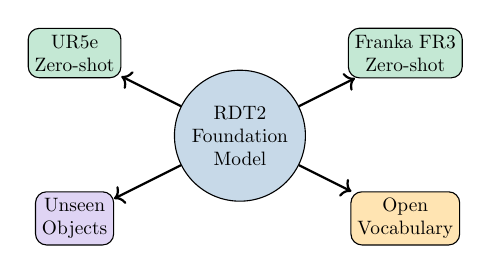
\begin{tikzpicture}[scale=0.7, transform shape]
                % Central node
                \node[draw, circle, fill=qwenblue!30, minimum size=2cm, align=center] (rdt2) at (0,0) {RDT2\\Foundation\\Model};

                % Surrounding capabilities
                \node[draw, rounded corners, fill=rdtgreen!30, align=center] (ur5e) at (-3, 1.5) {UR5e\\Zero-shot};
                \node[draw, rounded corners, fill=rdtgreen!30, align=center] (franka) at (3, 1.5) {Franka FR3\\Zero-shot};
                \node[draw, rounded corners, fill=vqpurple!30, align=center] (unseen) at (-3, -1.5) {Unseen\\Objects};
                \node[draw, rounded corners, fill=actionorange!30, align=center] (lang) at (3, -1.5) {Open\\Vocabulary};

                % Arrows
                \draw[->, thick] (rdt2) -- (ur5e);
                \draw[->, thick] (rdt2) -- (franka);
                \draw[->, thick] (rdt2) -- (unseen);
                \draw[->, thick] (rdt2) -- (lang);
            \end{tikzpicture}
        \end{column}
    \end{columns}
\end{frame}

\begin{frame}{Model Variants Overview}
    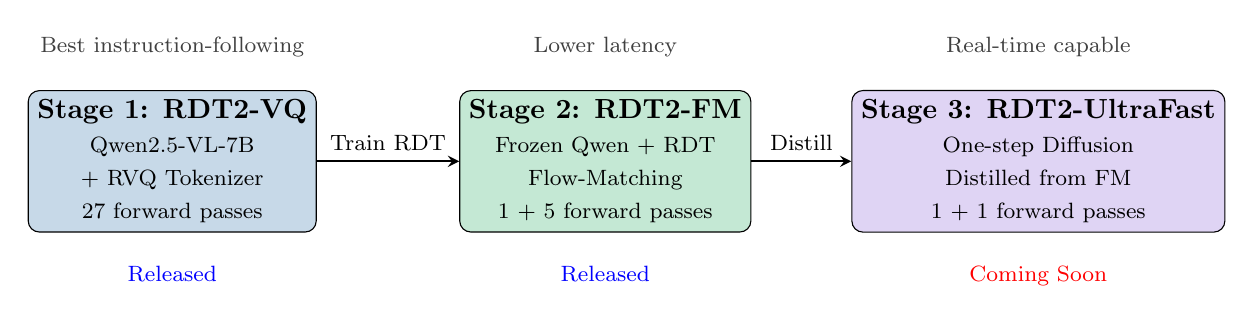
\begin{tikzpicture}[
        stage/.style={draw, rounded corners, minimum width=3.5cm, minimum height=1.5cm, align=center},
        arrow/.style={->, thick, >=stealth}
    ]
        % Stage 1
        \node[stage, fill=qwenblue!30] (vq) at (0, 0) {
            \textbf{Stage 1: RDT2-VQ}\\
            \footnotesize Qwen2.5-VL-7B\\
            \footnotesize + RVQ Tokenizer\\
            \footnotesize 27 forward passes
        };

        % Stage 2
        \node[stage, fill=rdtgreen!30] (fm) at (5.5, 0) {
            \textbf{Stage 2: RDT2-FM}\\
            \footnotesize Frozen Qwen + RDT\\
            \footnotesize Flow-Matching\\
            \footnotesize 1 + 5 forward passes
        };

        % Stage 3
        \node[stage, fill=vqpurple!30] (ultra) at (11, 0) {
            \textbf{Stage 3: RDT2-UltraFast}\\
            \footnotesize One-step Diffusion\\
            \footnotesize Distilled from FM\\
            \footnotesize 1 + 1 forward passes
        };

        % Arrows
        \draw[arrow] (vq) -- (fm) node[midway, above] {\footnotesize Train RDT};
        \draw[arrow] (fm) -- (ultra) node[midway, above] {\footnotesize Distill};

        % Status labels
        \node[below=0.3cm of vq, text=blue] {\footnotesize Released};
        \node[below=0.3cm of fm, text=blue] {\footnotesize Released};
        \node[below=0.3cm of ultra, text=red] {\footnotesize Coming Soon};

        % Performance indicators
        \node[above=0.3cm of vq, text=darkgray] {\footnotesize Best instruction-following};
        \node[above=0.3cm of fm, text=darkgray] {\footnotesize Lower latency};
        \node[above=0.3cm of ultra, text=darkgray] {\footnotesize Real-time capable};
    \end{tikzpicture}
\end{frame}

%==============================================================================
\section{UMI Hardware \& Data Collection}
%==============================================================================

\begin{frame}{UMI Hardware Platform}
    \begin{columns}
        \begin{column}{0.5\textwidth}
            \textbf{Hardware Redesign:}
            \begin{itemize}
                \item \textbf{Material}: Nylon 66 + Glass fiber (CNC machined)
                \item Previous: 3D printed (fragile)
                \item \textbf{Tracking}: HTC VIVE Tracker 3.0
                \item Previous: SLAM (unreliable in texture-less environments)
            \end{itemize}

            \vspace{0.3cm}
            \textbf{Key Benefit:}
            \begin{itemize}
                \item Unified end-effector design
                \item Minimizes embodiment gap
                \item Plug-and-play deployment
            \end{itemize}
        \end{column}
        \begin{column}{0.5\textwidth}
            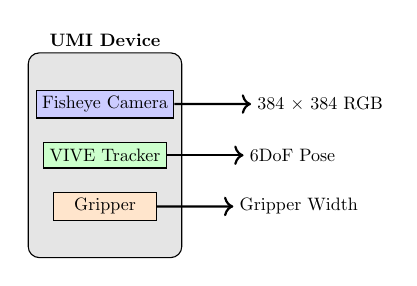
\begin{tikzpicture}[scale=0.65, transform shape]
                % UMI device
                \node[draw, rounded corners, fill=gray!20, minimum width=3cm, minimum height=4cm] (umi) at (0, 0) {};
                \node[above] at (umi.north) {\textbf{UMI Device}};

                % Components
                \node[draw, fill=blue!20, minimum width=2cm, minimum height=0.5cm] (cam) at (0, 1) {Fisheye Camera};
                \node[draw, fill=green!20, minimum width=2cm, minimum height=0.5cm] (tracker) at (0, 0) {VIVE Tracker};
                \node[draw, fill=orange!20, minimum width=2cm, minimum height=0.5cm] (gripper) at (0, -1) {Gripper};

                % Outputs
                \node[right=1.5cm of cam] (img) {384 $\times$ 384 RGB};
                \node[right=1.5cm of tracker] (pose) {6DoF Pose};
                \node[right=1.5cm of gripper] (width) {Gripper Width};

                \draw[->, thick] (cam) -- (img);
                \draw[->, thick] (tracker) -- (pose);
                \draw[->, thick] (gripper) -- (width);
            \end{tikzpicture}
        \end{column}
    \end{columns}
\end{frame}

\begin{frame}{Data Collection Scale}
    \begin{columns}
        \begin{column}{0.5\textwidth}
            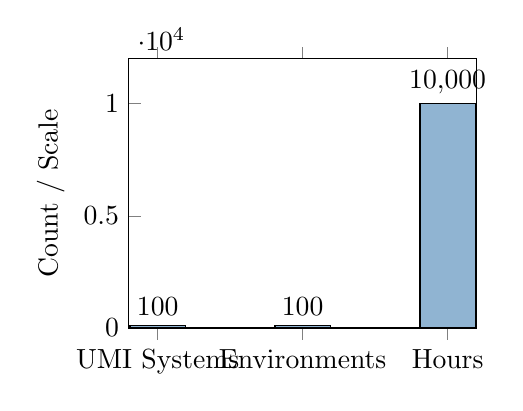
\begin{tikzpicture}
                \begin{axis}[
                    ybar,
                    symbolic x coords={UMI Systems, Environments, Hours},
                    xtick=data,
                    ylabel={Count / Scale},
                    ymin=0,
                    ymax=12000,
                    bar width=20pt,
                    nodes near coords,
                    width=6cm,
                    height=5cm
                ]
                \addplot[fill=qwenblue!60] coordinates {
                    (UMI Systems, 100)
                    (Environments, 100)
                    (Hours, 10000)
                };
                \end{axis}
            \end{tikzpicture}
        \end{column}
        \begin{column}{0.5\textwidth}
            \textbf{Collection Statistics:}
            \begin{itemize}
                \item $\sim$100 UMI systems manufactured
                \item 100+ real home/office environments
                \item 10,000+ hours of manipulation video
                \item $\sim$1/10 cost vs teleoperation
                \item 5$\times$ faster collection speed
            \end{itemize}

            \vspace{0.3cm}
            \textbf{Excluded Tasks:}
            \begin{itemize}
                \item Water contact
                \item Heat contact
                \item Five-finger dexterity
                \item Large consumable tasks
            \end{itemize}
        \end{column}
    \end{columns}
\end{frame}

\begin{frame}{WebDataset TAR Format}
    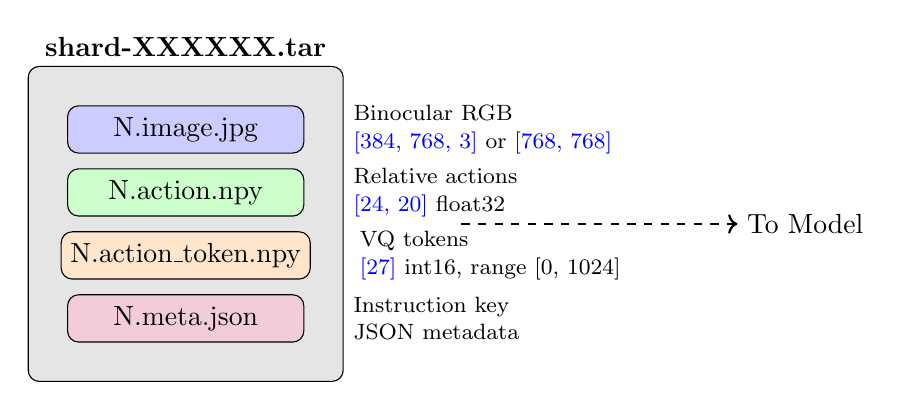
\begin{tikzpicture}[
        file/.style={draw, rounded corners, fill=white, minimum width=3cm, minimum height=0.6cm, align=center},
        shard/.style={draw, rounded corners, fill=gray!20, minimum width=4cm, minimum height=4cm}
    ]
        % TAR shard
        \node[shard] (tar) at (0, 0) {};
        \node[above] at (tar.north) {\textbf{shard-XXXXXX.tar}};

        % Files inside
        \node[file, fill=blue!20] (img) at (0, 1.2) {N.image.jpg};
        \node[file, fill=green!20] (act) at (0, 0.4) {N.action.npy};
        \node[file, fill=orange!20] (tok) at (0, -0.4) {N.action\_token.npy};
        \node[file, fill=purple!20] (meta) at (0, -1.2) {N.meta.json};

        % Descriptions
        \node[right=0.5cm of img, align=left] {\footnotesize Binocular RGB\\[-2pt] \footnotesize \dimension{384, 768, 3} or \dimension{768, 768}};
        \node[right=0.5cm of act, align=left] {\footnotesize Relative actions\\[-2pt] \footnotesize \dimension{24, 20} float32};
        \node[right=0.5cm of tok, align=left] {\footnotesize VQ tokens\\[-2pt] \footnotesize \dimension{27} int16, range [0, 1024]};
        \node[right=0.5cm of meta, align=left] {\footnotesize Instruction key\\[-2pt] \footnotesize JSON metadata};

        % Arrow showing flow
        \node[right=5cm of tar] (model) {To Model};
        \draw[->, thick, dashed] (3.5, 0) -- (model);
    \end{tikzpicture}
\end{frame}

%==============================================================================
\section{Action Representation}
%==============================================================================

\begin{frame}{Action Dimensions: 20-D Bimanual Structure}
    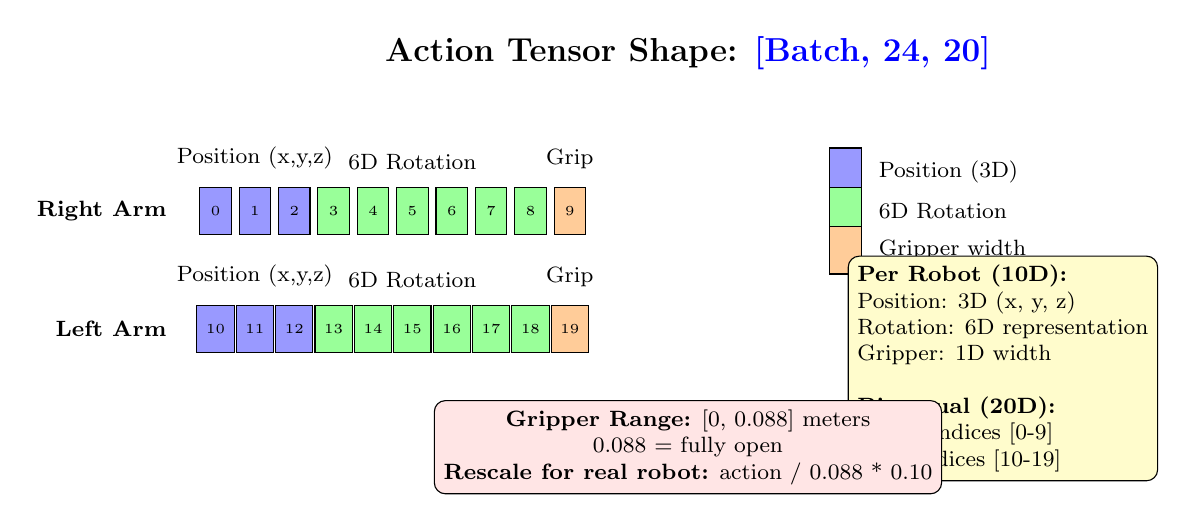
\begin{tikzpicture}[
        dim/.style={draw, minimum width=0.4cm, minimum height=0.6cm, font=\tiny},
        label/.style={font=\footnotesize}
    ]
        % Title
        \node[font=\large\bfseries] at (6, 4) {Action Tensor Shape: \dimension{Batch, 24, 20}};

        % Right arm
        \node[label, anchor=east] at (-0.5, 2) {\textbf{Right Arm}};

        % Position indices 0-2
        \foreach \i in {0,1,2} {
            \node[dim, fill=blue!40] (r\i) at (\i*0.5, 2) {\i};
        }
        \node[above=0.1cm of r1] {\footnotesize Position (x,y,z)};

        % Rotation indices 3-8
        \foreach \i in {3,4,5,6,7,8} {
            \node[dim, fill=green!40] (r\i) at (\i*0.5, 2) {\i};
        }
        \node[above=0.1cm of r5] {\footnotesize 6D Rotation};

        % Gripper index 9
        \node[dim, fill=orange!40] (r9) at (4.5, 2) {9};
        \node[above=0.1cm of r9] {\footnotesize Grip};

        % Left arm
        \node[label, anchor=east] at (-0.5, 0.5) {\textbf{Left Arm}};

        % Position indices 10-12
        \foreach \i in {10,11,12} {
            \pgfmathtruncatemacro{\x}{\i-10}
            \node[dim, fill=blue!40] (l\i) at (\x*0.5, 0.5) {\i};
        }
        \node[above=0.1cm of l11] {\footnotesize Position (x,y,z)};

        % Rotation indices 13-18
        \foreach \i in {13,14,15,16,17,18} {
            \pgfmathtruncatemacro{\x}{\i-10}
            \node[dim, fill=green!40] (l\i) at (\x*0.5, 0.5) {\i};
        }
        \node[above=0.1cm of l15] {\footnotesize 6D Rotation};

        % Gripper index 19
        \node[dim, fill=orange!40] (l19) at (4.5, 0.5) {19};
        \node[above=0.1cm of l19] {\footnotesize Grip};

        % Legend
        \node[dim, fill=blue!40] at (8, 2.5) {};
        \node[right, font=\footnotesize] at (8.3, 2.5) {Position (3D)};
        \node[dim, fill=green!40] at (8, 2) {};
        \node[right, font=\footnotesize] at (8.3, 2) {6D Rotation};
        \node[dim, fill=orange!40] at (8, 1.5) {};
        \node[right, font=\footnotesize] at (8.3, 1.5) {Gripper width};

        % Summary box
        \node[draw, rounded corners, fill=yellow!20, align=left, font=\footnotesize] at (10, 0) {
            \textbf{Per Robot (10D):}\\
            Position: 3D (x, y, z)\\
            Rotation: 6D representation\\
            Gripper: 1D width\\
            \\
            \textbf{Bimanual (20D):}\\
            Right: indices [0-9]\\
            Left: indices [10-19]
        };

        % Gripper range note
        \node[draw, rounded corners, fill=red!10, align=center, font=\footnotesize] at (6, -1) {
            \textbf{Gripper Range:} [0, 0.088] meters\\
            0.088 = fully open\\
            \textbf{Rescale for real robot:} action / 0.088 * 0.10
        };
    \end{tikzpicture}
\end{frame}

\begin{frame}{6D Rotation Representation}
    \begin{columns}
        \begin{column}{0.5\textwidth}
            \textbf{Why 6D instead of quaternion/euler?}
            \begin{itemize}
                \item Continuous representation
                \item No gimbal lock
                \item Easier to learn for neural networks
                \item Geodesic loss computation
            \end{itemize}

            \vspace{0.3cm}
            \textbf{Conversion: 6D $\rightarrow$ 3$\times$3 Matrix}
            \begin{align*}
                \mathbf{a}_1 &= \text{rot6d}[0:3] \\
                \mathbf{a}_2 &= \text{rot6d}[3:6] \\
                \mathbf{b}_1 &= \text{normalize}(\mathbf{a}_1) \\
                \mathbf{b}_2 &= \text{normalize}(\mathbf{a}_2 - (\mathbf{b}_1 \cdot \mathbf{a}_2)\mathbf{b}_1) \\
                \mathbf{b}_3 &= \mathbf{b}_1 \times \mathbf{b}_2 \\
                R &= [\mathbf{b}_1, \mathbf{b}_2, \mathbf{b}_3]
            \end{align*}
        \end{column}
        \begin{column}{0.5\textwidth}
            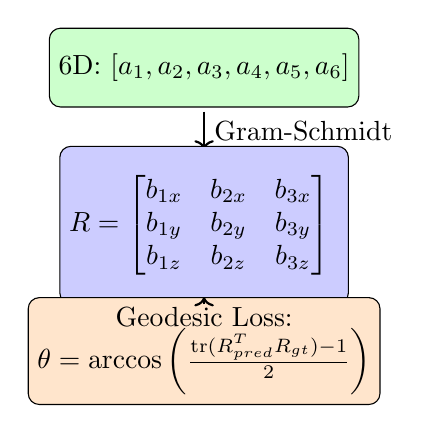
\begin{tikzpicture}[scale=0.8]
                % 6D vector
                \node[draw, rounded corners, fill=green!20, minimum width=3cm, minimum height=1cm] (rot6d) at (0, 3) {6D: $[a_1, a_2, a_3, a_4, a_5, a_6]$};

                % Arrow
                \draw[->, thick] (0, 2.3) -- (0, 1.7) node[midway, right] {Gram-Schmidt};

                % 3x3 Matrix
                \node[draw, rounded corners, fill=blue!20, minimum width=3cm, minimum height=2cm, align=center] (mat) at (0, 0.5) {
                    $R = \begin{bmatrix} b_{1x} & b_{2x} & b_{3x} \\ b_{1y} & b_{2y} & b_{3y} \\ b_{1z} & b_{2z} & b_{3z} \end{bmatrix}$
                };

                % Geodesic loss
                \node[draw, rounded corners, fill=orange!20, minimum width=3cm, minimum height=1cm, align=center] (loss) at (0, -1.5) {
                    Geodesic Loss:\\
                    $\theta = \arccos\left(\frac{\text{tr}(R_{pred}^T R_{gt}) - 1}{2}\right)$
                };

                \draw[->, thick] (mat) -- (loss);
            \end{tikzpicture}
        \end{column}
    \end{columns}
\end{frame}

\begin{frame}{Action Chunk: Temporal Structure}
    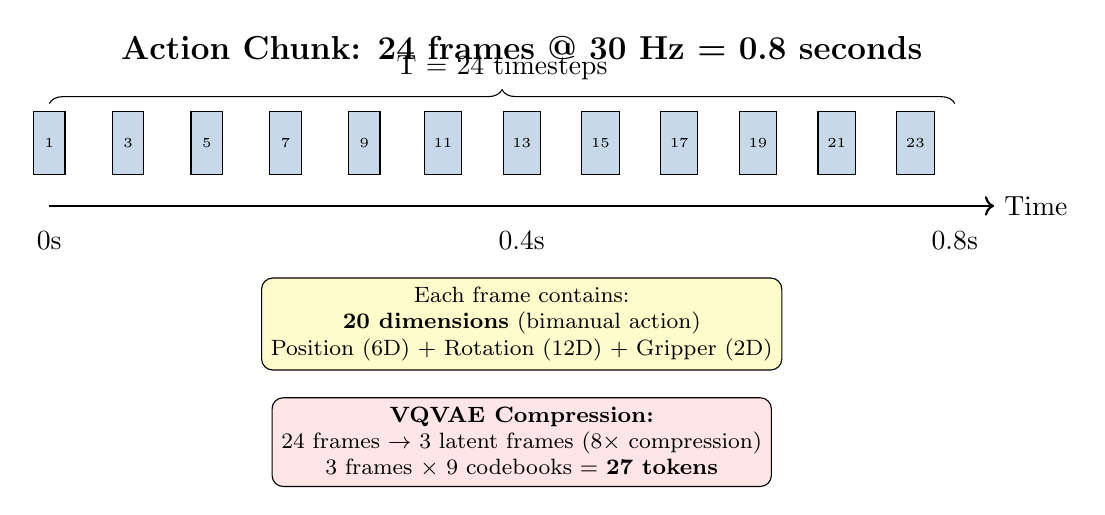
\begin{tikzpicture}[
        frame/.style={draw, minimum width=0.4cm, minimum height=0.8cm, font=\tiny}
    ]
        % Title
        \node[font=\large\bfseries] at (6, 4) {Action Chunk: 24 frames @ 30 Hz = 0.8 seconds};

        % Timeline
        \draw[thick, ->] (0, 2) -- (12, 2) node[right] {Time};

        % Frames
        \foreach \i in {0,1,2,3,4,5,6,7,8,9,10,11,12,13,14,15,16,17,18,19,20,21,22,23} {
            \pgfmathtruncatemacro{\x}{\i * 0.5}
            \node[frame, fill=qwenblue!30] at (\x, 2.8) {\i};
        }

        % Time labels
        \node[below] at (0, 1.8) {0s};
        \node[below] at (6, 1.8) {0.4s};
        \node[below] at (11.5, 1.8) {0.8s};

        % Dimension annotation
        \draw[decorate, decoration={brace, amplitude=5pt}] (0, 3.3) -- (11.5, 3.3)
            node[midway, above=5pt] {T = 24 timesteps};

        % Each frame content
        \node[draw, rounded corners, fill=yellow!20, align=center, font=\footnotesize] at (6, 0.5) {
            Each frame contains:\\
            \textbf{20 dimensions} (bimanual action)\\
            Position (6D) + Rotation (12D) + Gripper (2D)
        };

        % Compression note
        \node[draw, rounded corners, fill=red!10, align=center, font=\footnotesize] at (6, -1) {
            \textbf{VQVAE Compression:}\\
            24 frames $\rightarrow$ 3 latent frames (8$\times$ compression)\\
            3 frames $\times$ 9 codebooks = \textbf{27 tokens}
        };
    \end{tikzpicture}
\end{frame}

%==============================================================================
\section{VQVAE Action Tokenizer}
%==============================================================================

\begin{frame}{VQVAE Overview: Action $\rightarrow$ Tokens}
    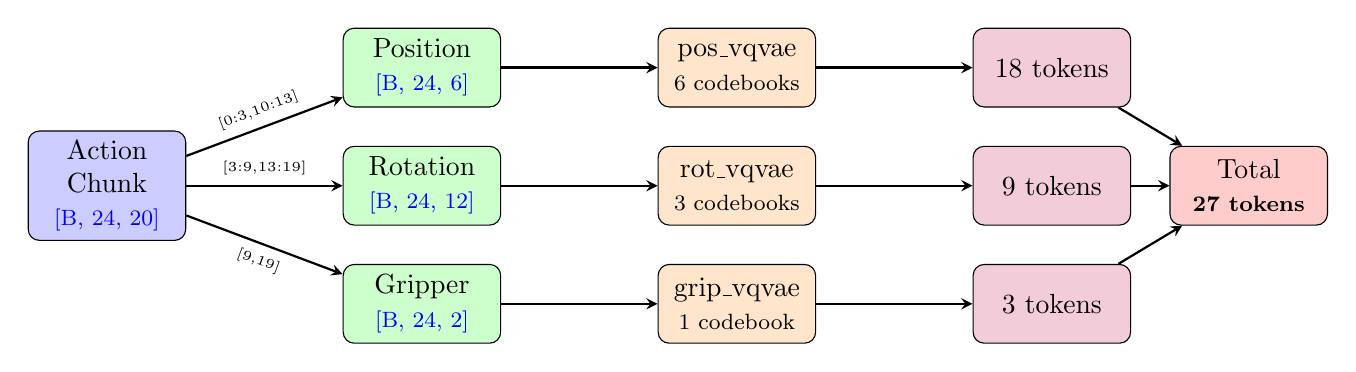
\begin{tikzpicture}[
        block/.style={draw, rounded corners, minimum width=2cm, minimum height=1cm, align=center},
        arrow/.style={->, thick, >=stealth}
    ]
        % Input
        \node[block, fill=blue!20] (input) at (0, 0) {Action\\Chunk\\{\footnotesize\dimension{B, 24, 20}}};

        % MultiVQVAE splits
        \node[block, fill=green!20] (pos) at (4, 1.5) {Position\\{\footnotesize\dimension{B, 24, 6}}};
        \node[block, fill=green!20] (rot) at (4, 0) {Rotation\\{\footnotesize\dimension{B, 24, 12}}};
        \node[block, fill=green!20] (grip) at (4, -1.5) {Gripper\\{\footnotesize\dimension{B, 24, 2}}};

        % Individual VQVAEs
        \node[block, fill=orange!20] (posvq) at (8, 1.5) {pos\_vqvae\\{\footnotesize 6 codebooks}};
        \node[block, fill=orange!20] (rotvq) at (8, 0) {rot\_vqvae\\{\footnotesize 3 codebooks}};
        \node[block, fill=orange!20] (gripvq) at (8, -1.5) {grip\_vqvae\\{\footnotesize 1 codebook}};

        % Tokens
        \node[block, fill=purple!20] (postok) at (12, 1.5) {18 tokens};
        \node[block, fill=purple!20] (rottok) at (12, 0) {9 tokens};
        \node[block, fill=purple!20] (griptok) at (12, -1.5) {3 tokens};

        % Output
        \node[block, fill=red!20] (output) at (14.5, 0) {Total\\{\footnotesize\textbf{27 tokens}}};

        % Arrows
        \draw[arrow] (input) -- (pos) node[midway, above, sloped, font=\tiny] {[0:3,10:13]};
        \draw[arrow] (input) -- (rot) node[midway, above, sloped, font=\tiny] {[3:9,13:19]};
        \draw[arrow] (input) -- (grip) node[midway, below, sloped, font=\tiny] {[9,19]};

        \draw[arrow] (pos) -- (posvq);
        \draw[arrow] (rot) -- (rotvq);
        \draw[arrow] (grip) -- (gripvq);

        \draw[arrow] (posvq) -- (postok);
        \draw[arrow] (rotvq) -- (rottok);
        \draw[arrow] (gripvq) -- (griptok);

        \draw[arrow] (postok) -- (output);
        \draw[arrow] (rottok) -- (output);
        \draw[arrow] (griptok) -- (output);
    \end{tikzpicture}
\end{frame}

\begin{frame}{Single VQVAE Architecture}
    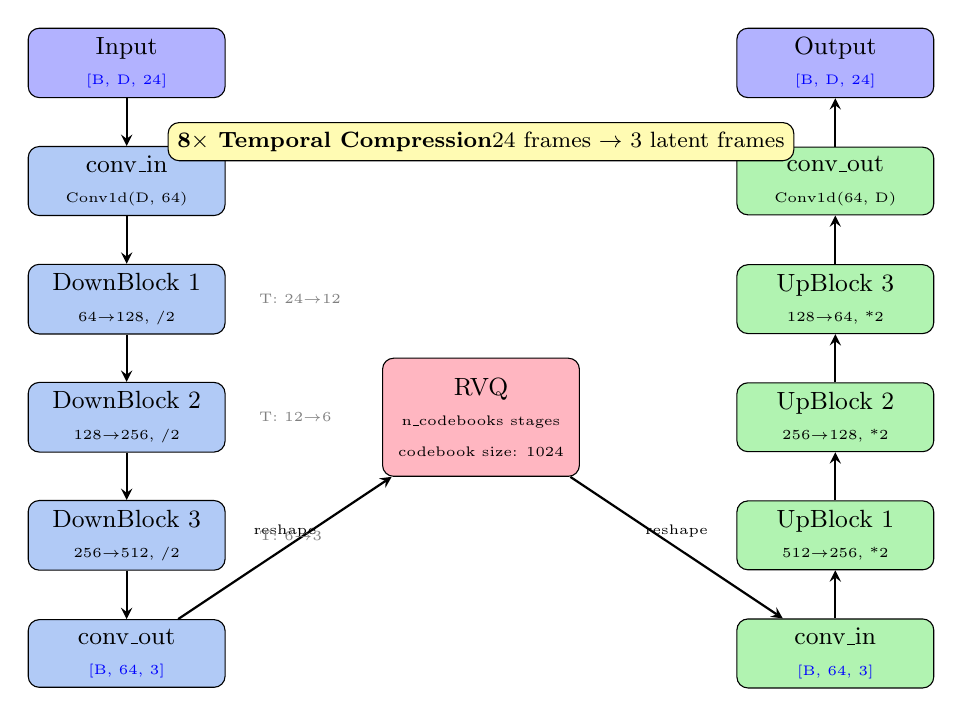
\begin{tikzpicture}[
        block/.style={draw, rounded corners, minimum width=2.5cm, minimum height=0.8cm, align=center, font=\small},
        arrow/.style={->, thick, >=stealth}
    ]
        % Encoder path
        \node[block, fill=blue!30] (in) at (0, 3) {Input\\{\tiny\dimension{B, D, 24}}};

        \node[block, fill=encoderblue!50] (conv1) at (0, 1.5) {conv\_in\\{\tiny Conv1d(D, 64)}};

        \node[block, fill=encoderblue!50] (down1) at (0, 0) {DownBlock 1\\{\tiny 64$\rightarrow$128, /2}};

        \node[block, fill=encoderblue!50] (down2) at (0, -1.5) {DownBlock 2\\{\tiny 128$\rightarrow$256, /2}};

        \node[block, fill=encoderblue!50] (down3) at (0, -3) {DownBlock 3\\{\tiny 256$\rightarrow$512, /2}};

        \node[block, fill=encoderblue!50] (cout) at (0, -4.5) {conv\_out\\{\tiny\dimension{B, 64, 3}}};

        % VQ
        \node[block, fill=codebookpink, minimum height=1.5cm] (vq) at (4.5, -1.5) {
            RVQ\\
            {\tiny n\_codebooks stages}\\
            {\tiny codebook size: 1024}
        };

        % Decoder path
        \node[block, fill=decodergreen!70] (din) at (9, -4.5) {conv\_in\\{\tiny\dimension{B, 64, 3}}};

        \node[block, fill=decodergreen!70] (up1) at (9, -3) {UpBlock 1\\{\tiny 512$\rightarrow$256, *2}};

        \node[block, fill=decodergreen!70] (up2) at (9, -1.5) {UpBlock 2\\{\tiny 256$\rightarrow$128, *2}};

        \node[block, fill=decodergreen!70] (up3) at (9, 0) {UpBlock 3\\{\tiny 128$\rightarrow$64, *2}};

        \node[block, fill=decodergreen!70] (dout) at (9, 1.5) {conv\_out\\{\tiny Conv1d(64, D)}};

        \node[block, fill=blue!30] (out) at (9, 3) {Output\\{\tiny\dimension{B, D, 24}}};

        % Arrows - Encoder
        \draw[arrow] (in) -- (conv1);
        \draw[arrow] (conv1) -- (down1);
        \draw[arrow] (down1) -- (down2);
        \draw[arrow] (down2) -- (down3);
        \draw[arrow] (down3) -- (cout);

        % Arrows - VQ
        \draw[arrow] (cout) -- (vq) node[midway, above, font=\tiny] {reshape};
        \draw[arrow] (vq) -- (din) node[midway, above, font=\tiny] {reshape};

        % Arrows - Decoder
        \draw[arrow] (din) -- (up1);
        \draw[arrow] (up1) -- (up2);
        \draw[arrow] (up2) -- (up3);
        \draw[arrow] (up3) -- (dout);
        \draw[arrow] (dout) -- (out);

        % Dimension annotations
        \node[right=0.3cm of down1, font=\tiny, text=gray] {T: 24$\rightarrow$12};
        \node[right=0.3cm of down2, font=\tiny, text=gray] {T: 12$\rightarrow$6};
        \node[right=0.3cm of down3, font=\tiny, text=gray] {T: 6$\rightarrow$3};

        % 8x compression note
        \node[draw, rounded corners, fill=yellow!30, font=\footnotesize] at (4.5, 2) {
            \textbf{8$\times$ Temporal Compression}\\
            24 frames $\rightarrow$ 3 latent frames
        };
    \end{tikzpicture}
\end{frame}

\begin{frame}{Residual Vector Quantization (RVQ)}
    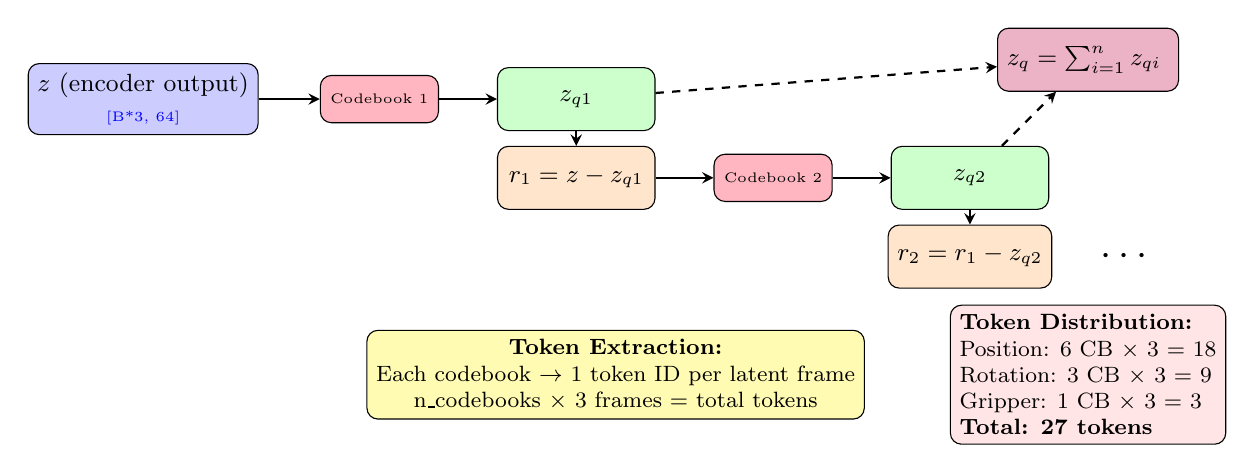
\begin{tikzpicture}[
        block/.style={draw, rounded corners, minimum width=2cm, minimum height=0.8cm, align=center, font=\small},
        cb/.style={draw, rounded corners, fill=codebookpink, minimum width=1.5cm, minimum height=0.6cm, font=\tiny},
        arrow/.style={->, thick, >=stealth}
    ]
        % Input
        \node[block, fill=blue!20] (z) at (0, 0) {$z$ (encoder output)\\{\tiny\dimension{B*3, 64}}};

        % Stage 1
        \node[cb] (cb1) at (3, 0) {Codebook 1};
        \node[block, fill=green!20] (zq1) at (5.5, 0) {$z_{q1}$};
        \node[block, fill=orange!20] (r1) at (5.5, -1) {$r_1 = z - z_{q1}$};

        % Stage 2
        \node[cb] (cb2) at (8, -1) {Codebook 2};
        \node[block, fill=green!20] (zq2) at (10.5, -1) {$z_{q2}$};
        \node[block, fill=orange!20] (r2) at (10.5, -2) {$r_2 = r_1 - z_{q2}$};

        % Stage n
        \node[font=\Large] at (12.5, -2) {$\cdots$};

        % Final
        \node[block, fill=purple!30] (final) at (12, 0.5) {
            $z_q = \sum_{i=1}^{n} z_{qi}$
        };

        % Arrows
        \draw[arrow] (z) -- (cb1);
        \draw[arrow] (cb1) -- (zq1);
        \draw[arrow] (zq1) -- (r1);
        \draw[arrow] (r1) -- (cb2);
        \draw[arrow] (cb2) -- (zq2);
        \draw[arrow] (zq2) -- (r2);

        \draw[arrow, dashed] (zq1) -- (final);
        \draw[arrow, dashed] (zq2) -- (final);

        % Token extraction
        \node[draw, rounded corners, fill=yellow!30, align=center, font=\footnotesize] at (6, -3.5) {
            \textbf{Token Extraction:}\\
            Each codebook $\rightarrow$ 1 token ID per latent frame\\
            n\_codebooks $\times$ 3 frames = total tokens
        };

        % Token counts
        \node[draw, rounded corners, fill=red!10, align=left, font=\footnotesize] at (12, -3.5) {
            \textbf{Token Distribution:}\\
            Position: 6 CB $\times$ 3 = 18\\
            Rotation: 3 CB $\times$ 3 = 9\\
            Gripper: 1 CB $\times$ 3 = 3\\
            \textbf{Total: 27 tokens}
        };
    \end{tikzpicture}
\end{frame}

\begin{frame}{Vector Quantizer: Core Mechanism}
    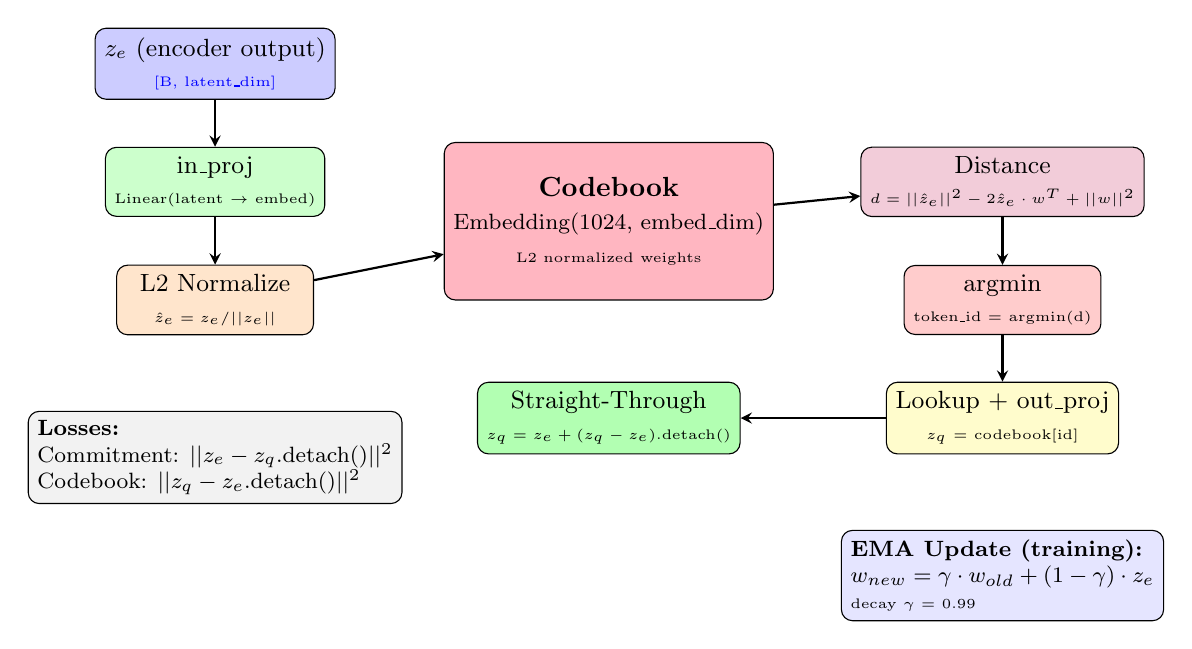
\begin{tikzpicture}[
        block/.style={draw, rounded corners, minimum width=2.5cm, minimum height=0.8cm, align=center, font=\small},
        arrow/.style={->, thick, >=stealth}
    ]
        % Input projection
        \node[block, fill=blue!20] (input) at (0, 2) {$z_e$ (encoder output)\\{\tiny\dimension{B, latent\_dim}}};

        \node[block, fill=green!20] (proj) at (0, 0.5) {in\_proj\\{\tiny Linear(latent $\rightarrow$ embed)}};

        \node[block, fill=orange!20] (norm) at (0, -1) {L2 Normalize\\{\tiny $\hat{z}_e = z_e / ||z_e||$}};

        % Codebook
        \node[draw, rounded corners, fill=codebookpink, minimum width=3cm, minimum height=2cm, align=center] (cb) at (5, 0) {
            \textbf{Codebook}\\
            {\footnotesize Embedding(1024, embed\_dim)}\\
            {\tiny L2 normalized weights}
        };

        % Distance calculation
        \node[block, fill=purple!20] (dist) at (10, 0.5) {
            Distance\\
            {\tiny $d = ||\hat{z}_e||^2 - 2\hat{z}_e \cdot w^T + ||w||^2$}
        };

        % Argmin
        \node[block, fill=red!20] (argmin) at (10, -1) {argmin\\{\tiny token\_id = argmin(d)}};

        % Lookup
        \node[block, fill=yellow!20] (lookup) at (10, -2.5) {Lookup + out\_proj\\{\tiny $z_q$ = codebook[id]}};

        % Straight-through
        \node[block, fill=green!30] (st) at (5, -2.5) {
            Straight-Through\\
            {\tiny $z_q = z_e + (z_q - z_e)$.detach()}
        };

        % Arrows
        \draw[arrow] (input) -- (proj);
        \draw[arrow] (proj) -- (norm);
        \draw[arrow] (norm) -- (cb);
        \draw[arrow] (cb) -- (dist);
        \draw[arrow] (dist) -- (argmin);
        \draw[arrow] (argmin) -- (lookup);
        \draw[arrow] (lookup) -- (st);

        % Loss annotation
        \node[draw, rounded corners, fill=gray!10, align=left, font=\footnotesize] at (0, -3) {
            \textbf{Losses:}\\
            Commitment: $||z_e - z_q.\text{detach}()||^2$\\
            Codebook: $||z_q - z_e.\text{detach}()||^2$
        };

        % EMA update
        \node[draw, rounded corners, fill=blue!10, align=left, font=\footnotesize] at (10, -4.5) {
            \textbf{EMA Update (training):}\\
            $w_{new} = \gamma \cdot w_{old} + (1-\gamma) \cdot z_e$\\
            {\tiny decay $\gamma$ = 0.99}
        };
    \end{tikzpicture}
\end{frame}

\begin{frame}{MultiVQVAE: Complete Dimension Flow}
    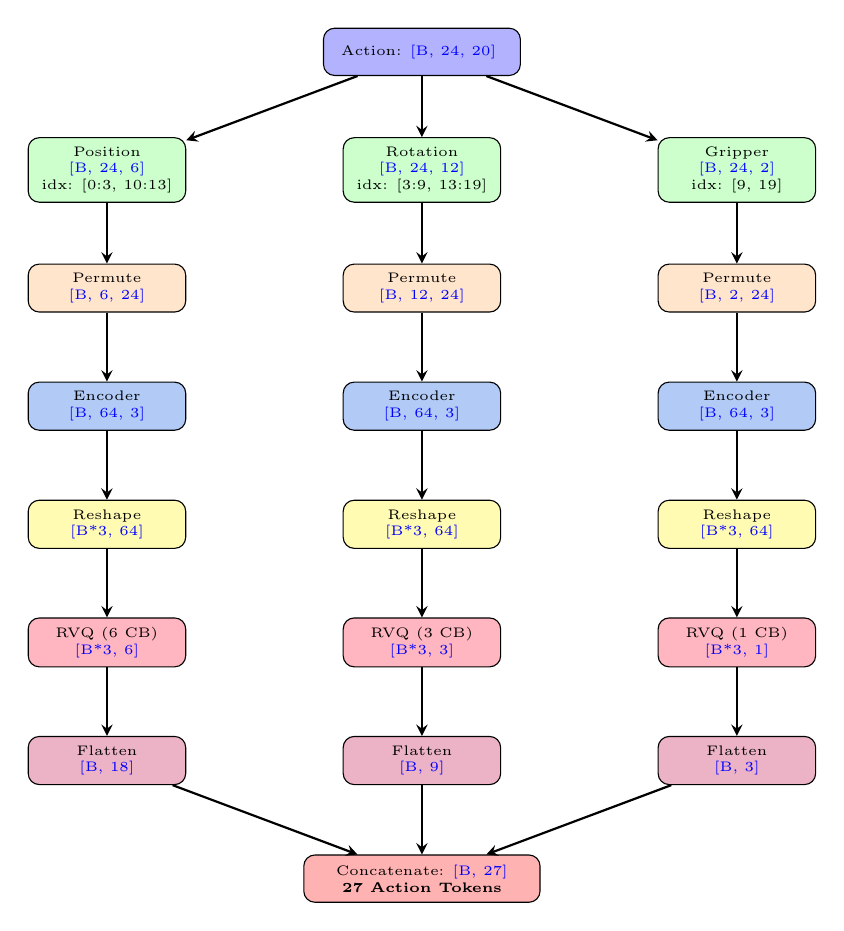
\begin{tikzpicture}[
        block/.style={draw, rounded corners, minimum height=0.6cm, align=center, font=\tiny},
        arrow/.style={->, thick, >=stealth}
    ]
        % Scale
        \def\scale{0.85}

        % Input action
        \node[block, fill=blue!30, minimum width=2.5cm] (in) at (0, 4) {
            Action: \dimension{B, 24, 20}
        };

        % Split
        \node[block, fill=green!20, minimum width=2cm] (pos) at (-4, 2.5) {
            Position\\
            \dimension{B, 24, 6}\\
            idx: [0:3, 10:13]
        };
        \node[block, fill=green!20, minimum width=2cm] (rot) at (0, 2.5) {
            Rotation\\
            \dimension{B, 24, 12}\\
            idx: [3:9, 13:19]
        };
        \node[block, fill=green!20, minimum width=2cm] (grip) at (4, 2.5) {
            Gripper\\
            \dimension{B, 24, 2}\\
            idx: [9, 19]
        };

        % Permute
        \node[block, fill=orange!20, minimum width=2cm] (posp) at (-4, 1) {
            Permute\\
            \dimension{B, 6, 24}
        };
        \node[block, fill=orange!20, minimum width=2cm] (rotp) at (0, 1) {
            Permute\\
            \dimension{B, 12, 24}
        };
        \node[block, fill=orange!20, minimum width=2cm] (gripp) at (4, 1) {
            Permute\\
            \dimension{B, 2, 24}
        };

        % Encoder output
        \node[block, fill=encoderblue!50, minimum width=2cm] (pose) at (-4, -0.5) {
            Encoder\\
            \dimension{B, 64, 3}
        };
        \node[block, fill=encoderblue!50, minimum width=2cm] (rote) at (0, -0.5) {
            Encoder\\
            \dimension{B, 64, 3}
        };
        \node[block, fill=encoderblue!50, minimum width=2cm] (gripe) at (4, -0.5) {
            Encoder\\
            \dimension{B, 64, 3}
        };

        % Reshape for VQ
        \node[block, fill=yellow!30, minimum width=2cm] (posr) at (-4, -2) {
            Reshape\\
            \dimension{B*3, 64}
        };
        \node[block, fill=yellow!30, minimum width=2cm] (rotr) at (0, -2) {
            Reshape\\
            \dimension{B*3, 64}
        };
        \node[block, fill=yellow!30, minimum width=2cm] (gripr) at (4, -2) {
            Reshape\\
            \dimension{B*3, 64}
        };

        % RVQ
        \node[block, fill=codebookpink, minimum width=2cm] (posrvq) at (-4, -3.5) {
            RVQ (6 CB)\\
            \dimension{B*3, 6}
        };
        \node[block, fill=codebookpink, minimum width=2cm] (rotrvq) at (0, -3.5) {
            RVQ (3 CB)\\
            \dimension{B*3, 3}
        };
        \node[block, fill=codebookpink, minimum width=2cm] (griprvq) at (4, -3.5) {
            RVQ (1 CB)\\
            \dimension{B*3, 1}
        };

        % Flatten
        \node[block, fill=purple!30, minimum width=2cm] (posf) at (-4, -5) {
            Flatten\\
            \dimension{B, 18}
        };
        \node[block, fill=purple!30, minimum width=2cm] (rotf) at (0, -5) {
            Flatten\\
            \dimension{B, 9}
        };
        \node[block, fill=purple!30, minimum width=2cm] (gripf) at (4, -5) {
            Flatten\\
            \dimension{B, 3}
        };

        % Concatenate
        \node[block, fill=red!30, minimum width=3cm] (out) at (0, -6.5) {
            Concatenate: \dimension{B, 27}\\
            \textbf{27 Action Tokens}
        };

        % Arrows
        \draw[arrow] (in) -- (pos);
        \draw[arrow] (in) -- (rot);
        \draw[arrow] (in) -- (grip);

        \draw[arrow] (pos) -- (posp);
        \draw[arrow] (rot) -- (rotp);
        \draw[arrow] (grip) -- (gripp);

        \draw[arrow] (posp) -- (pose);
        \draw[arrow] (rotp) -- (rote);
        \draw[arrow] (gripp) -- (gripe);

        \draw[arrow] (pose) -- (posr);
        \draw[arrow] (rote) -- (rotr);
        \draw[arrow] (gripe) -- (gripr);

        \draw[arrow] (posr) -- (posrvq);
        \draw[arrow] (rotr) -- (rotrvq);
        \draw[arrow] (gripr) -- (griprvq);

        \draw[arrow] (posrvq) -- (posf);
        \draw[arrow] (rotrvq) -- (rotf);
        \draw[arrow] (griprvq) -- (gripf);

        \draw[arrow] (posf) -- (out);
        \draw[arrow] (rotf) -- (out);
        \draw[arrow] (gripf) -- (out);
    \end{tikzpicture}
\end{frame}

%==============================================================================
\section{RDT2-VQ Architecture}
%==============================================================================

\begin{frame}{RDT2-VQ: Overall Architecture}
    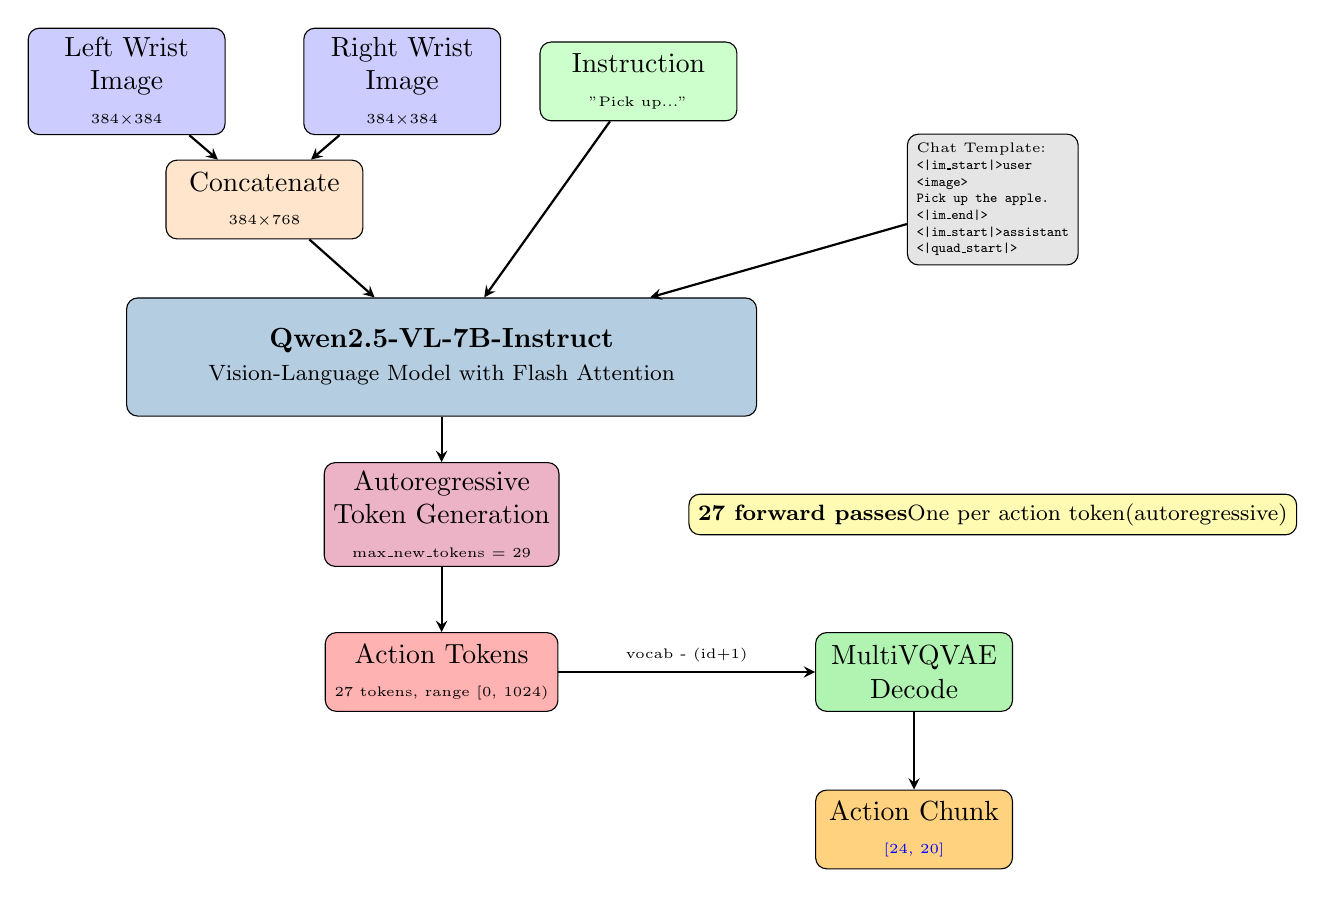
\begin{tikzpicture}[
        block/.style={draw, rounded corners, minimum width=2.5cm, minimum height=1cm, align=center},
        arrow/.style={->, thick, >=stealth}
    ]
        % Inputs
        \node[block, fill=blue!20] (img1) at (-1, 3) {Left Wrist\\Image\\{\tiny 384$\times$384}};
        \node[block, fill=blue!20] (img2) at (2.5, 3) {Right Wrist\\Image\\{\tiny 384$\times$384}};
        \node[block, fill=green!20] (instr) at (5.5, 3) {Instruction\\{\tiny "Pick up..."}};

        % Concatenate images
        \node[block, fill=orange!20] (concat) at (0.75, 1.5) {Concatenate\\{\tiny 384$\times$768}};

        % Qwen processor
        \node[block, fill=qwenblue!40, minimum width=8cm, minimum height=1.5cm] (qwen) at (3, -0.5) {
            \textbf{Qwen2.5-VL-7B-Instruct}\\
            {\footnotesize Vision-Language Model with Flash Attention}
        };

        % Chat template
        \node[draw, rounded corners, fill=gray!20, font=\tiny, align=left] (chat) at (10, 1.5) {
            Chat Template:\\
            \texttt{<|im\_start|>user}\\
            \texttt{<image>}\\
            \texttt{Pick up the apple.}\\
            \texttt{<|im\_end|>}\\
            \texttt{<|im\_start|>assistant}\\
            \texttt{<|quad\_start|>}
        };

        % Token generation
        \node[block, fill=purple!30] (gen) at (3, -2.5) {
            Autoregressive\\
            Token Generation\\
            {\tiny max\_new\_tokens = 29}
        };

        % Action tokens
        \node[block, fill=red!30] (tokens) at (3, -4.5) {
            Action Tokens\\
            {\tiny 27 tokens, range [0, 1024)}
        };

        % VQVAE decoder
        \node[block, fill=decodergreen!70] (vae) at (9, -4.5) {
            MultiVQVAE\\
            Decode
        };

        % Output
        \node[block, fill=actionorange!50] (out) at (9, -6.5) {
            Action Chunk\\
            {\tiny\dimension{24, 20}}
        };

        % Arrows
        \draw[arrow] (img1) -- (concat);
        \draw[arrow] (img2) -- (concat);
        \draw[arrow] (concat) -- (qwen);
        \draw[arrow] (instr) -- (qwen);
        \draw[arrow] (chat) -- (qwen);
        \draw[arrow] (qwen) -- (gen);
        \draw[arrow] (gen) -- (tokens);
        \draw[arrow] (tokens) -- (vae) node[midway, above, font=\tiny] {vocab - (id+1)};
        \draw[arrow] (vae) -- (out);

        % 27 forward passes note
        \node[draw, rounded corners, fill=yellow!30, font=\footnotesize] at (10, -2.5) {
            \textbf{27 forward passes}\\
            One per action token\\
            (autoregressive)
        };
    \end{tikzpicture}
\end{frame}

\begin{frame}{Token ID Conversion: VLA $\leftrightarrow$ VQVAE}
    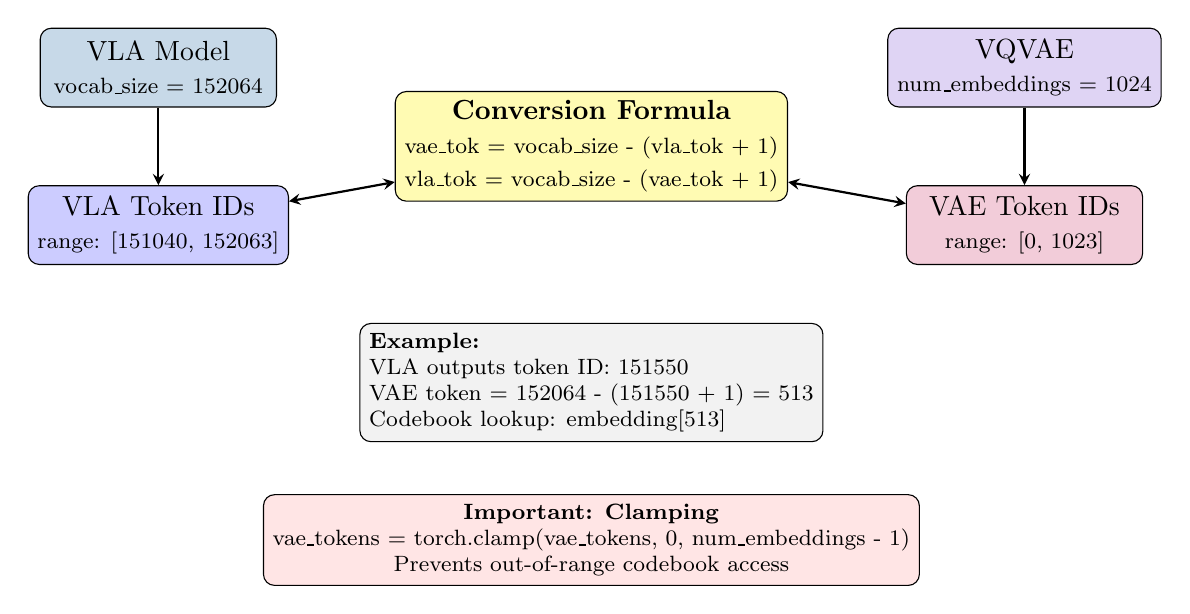
\begin{tikzpicture}[
        block/.style={draw, rounded corners, minimum width=3cm, minimum height=1cm, align=center},
        arrow/.style={->, thick, >=stealth}
    ]
        % VLA side
        \node[block, fill=qwenblue!30] (vla) at (0, 2) {
            VLA Model\\
            {\footnotesize vocab\_size = 152064}
        };

        \node[block, fill=blue!20] (vlatok) at (0, 0) {
            VLA Token IDs\\
            {\footnotesize range: [151040, 152063]}
        };

        % Conversion
        \node[block, fill=yellow!30, minimum width=4cm] (conv) at (5.5, 1) {
            \textbf{Conversion Formula}\\
            {\footnotesize vae\_tok = vocab\_size - (vla\_tok + 1)}\\
            {\footnotesize vla\_tok = vocab\_size - (vae\_tok + 1)}
        };

        % VQVAE side
        \node[block, fill=vqpurple!30] (vae) at (11, 2) {
            VQVAE\\
            {\footnotesize num\_embeddings = 1024}
        };

        \node[block, fill=purple!20] (vaetok) at (11, 0) {
            VAE Token IDs\\
            {\footnotesize range: [0, 1023]}
        };

        % Arrows
        \draw[arrow] (vla) -- (vlatok);
        \draw[arrow] (vae) -- (vaetok);
        \draw[arrow, <->] (vlatok) -- (conv);
        \draw[arrow, <->] (conv) -- (vaetok);

        % Example
        \node[draw, rounded corners, fill=gray!10, align=left, font=\footnotesize] at (5.5, -2) {
            \textbf{Example:}\\
            VLA outputs token ID: 151550\\
            VAE token = 152064 - (151550 + 1) = 513\\
            Codebook lookup: embedding[513]
        };

        % Clamping note
        \node[draw, rounded corners, fill=red!10, align=center, font=\footnotesize] at (5.5, -4) {
            \textbf{Important: Clamping}\\
            vae\_tokens = torch.clamp(vae\_tokens, 0, num\_embeddings - 1)\\
            Prevents out-of-range codebook access
        };
    \end{tikzpicture}
\end{frame}

\begin{frame}[fragile]{RDT2-VQ: Inference Code Flow}
\begin{lstlisting}[language=Python, title=utils.py: batch\_predict\_action()]
def batch_predict_action(model, processor, vae, normalizer, examples, ...):
    # 1. Preprocess images (concatenate left-right)
    images = [preprocess_data_from_umi(ex) for ex in examples]

    # 2. Apply optional JPEG compression (if trained with it)
    if apply_jpeg_compression:
        images = [jpeg_compress(img) for img in images]

    # 3. Build chat template with guidance tokens
    text = processor.apply_chat_template(messages)
    text += "<|im_start|>assistant\n<|quad_start|>"

    # 4. Generate action tokens (autoregressive)
    outputs = model.generate(inputs, max_new_tokens=valid_action_id_length + 2)

    # 5. Extract action token IDs (between markers)
    action_ids = extract_action_tokens(outputs)

    # 6. Convert VLA tokens to VAE tokens
    vae_tokens = vocab_size - (action_ids + 1)
    vae_tokens = torch.clamp(vae_tokens, 0, vae.num_embeddings - 1)

    # 7. Decode with VQVAE
    actions = vae.decode(vae_tokens)  # [B, 24, 20]

    # 8. Unnormalize
    actions = normalizer["action"].unnormalize(actions)

    return actions
\end{lstlisting}
\end{frame}

%==============================================================================
\section{RDT2-FM Architecture}
%==============================================================================

\begin{frame}{RDT2-FM: Flow-Matching Action Expert}
    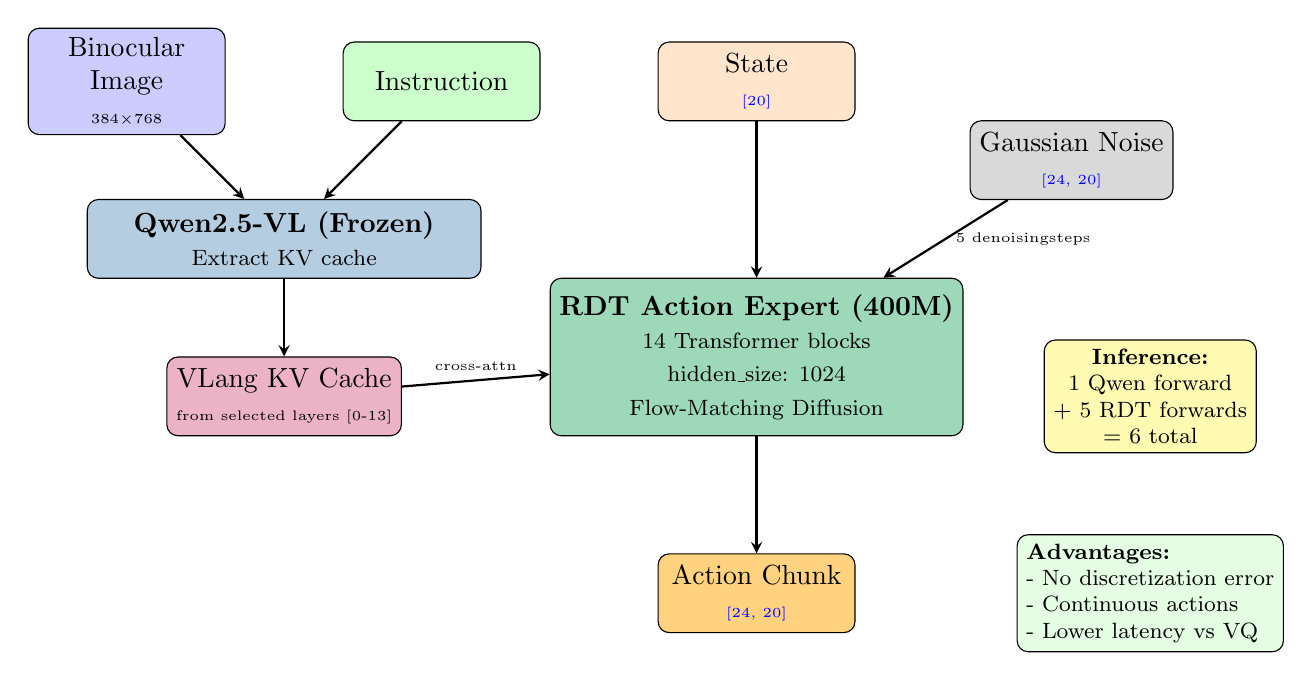
\begin{tikzpicture}[
        block/.style={draw, rounded corners, minimum width=2.5cm, minimum height=1cm, align=center},
        arrow/.style={->, thick, >=stealth}
    ]
        % Inputs
        \node[block, fill=blue!20] (img) at (-1, 3) {Binocular\\Image\\{\tiny 384$\times$768}};
        \node[block, fill=green!20] (instr) at (3, 3) {Instruction};
        \node[block, fill=orange!20] (state) at (7, 3) {State\\{\tiny\dimension{20}}};

        % Qwen (frozen)
        \node[block, fill=qwenblue!40, minimum width=5cm] (qwen) at (1, 1) {
            \textbf{Qwen2.5-VL (Frozen)}\\
            {\footnotesize Extract KV cache}
        };

        % KV cache
        \node[block, fill=purple!30] (kv) at (1, -1) {
            VLang KV Cache\\
            {\tiny from selected layers [0-13]}
        };

        % RDT
        \node[block, fill=rdtgreen!50, minimum width=5cm, minimum height=2cm] (rdt) at (7, -0.5) {
            \textbf{RDT Action Expert (400M)}\\
            {\footnotesize 14 Transformer blocks}\\
            {\footnotesize hidden\_size: 1024}\\
            {\footnotesize Flow-Matching Diffusion}
        };

        % Noise
        \node[block, fill=gray!30] (noise) at (11, 2) {
            Gaussian Noise\\
            {\tiny\dimension{24, 20}}
        };

        % Output
        \node[block, fill=actionorange!50] (out) at (7, -3.5) {
            Action Chunk\\
            {\tiny\dimension{24, 20}}
        };

        % Arrows
        \draw[arrow] (img) -- (qwen);
        \draw[arrow] (instr) -- (qwen);
        \draw[arrow] (qwen) -- (kv);
        \draw[arrow] (kv) -- (rdt) node[midway, above, font=\tiny] {cross-attn};
        \draw[arrow] (state) -- (rdt);
        \draw[arrow] (noise) -- (rdt) node[midway, right, font=\tiny] {5 denoising\\steps};
        \draw[arrow] (rdt) -- (out);

        % Forward passes note
        \node[draw, rounded corners, fill=yellow!30, font=\footnotesize, align=center] at (12, -1) {
            \textbf{Inference:}\\
            1 Qwen forward\\
            + 5 RDT forwards\\
            = 6 total
        };

        % Advantage
        \node[draw, rounded corners, fill=green!10, font=\footnotesize, align=left] at (12, -3.5) {
            \textbf{Advantages:}\\
            - No discretization error\\
            - Continuous actions\\
            - Lower latency vs VQ
        };
    \end{tikzpicture}
\end{frame}

\begin{frame}{RDT: Transformer Architecture}
    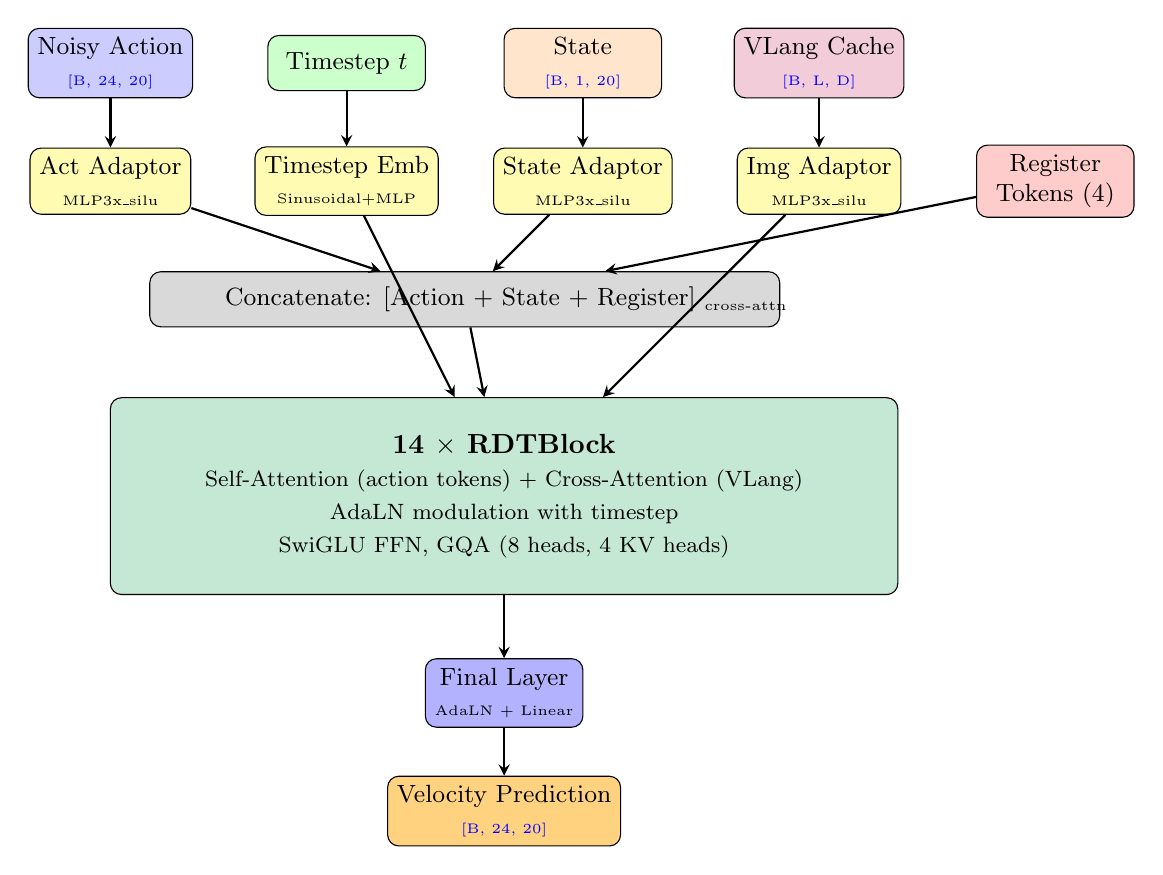
\begin{tikzpicture}[
        block/.style={draw, rounded corners, minimum width=2cm, minimum height=0.7cm, align=center, font=\small},
        arrow/.style={->, thick, >=stealth}
    ]
        % Inputs
        \node[block, fill=blue!20] (act) at (0, 5) {Noisy Action\\{\tiny\dimension{B, 24, 20}}};
        \node[block, fill=green!20] (t) at (3, 5) {Timestep $t$};
        \node[block, fill=orange!20] (state) at (6, 5) {State\\{\tiny\dimension{B, 1, 20}}};
        \node[block, fill=purple!20] (vlang) at (9, 5) {VLang Cache\\{\tiny\dimension{B, L, D}}};

        % Embeddings
        \node[block, fill=yellow!30] (actemb) at (0, 3.5) {Act Adaptor\\{\tiny MLP3x\_silu}};
        \node[block, fill=yellow!30] (temb) at (3, 3.5) {Timestep Emb\\{\tiny Sinusoidal+MLP}};
        \node[block, fill=yellow!30] (stemb) at (6, 3.5) {State Adaptor\\{\tiny MLP3x\_silu}};
        \node[block, fill=yellow!30] (imgemb) at (9, 3.5) {Img Adaptor\\{\tiny MLP3x\_silu}};

        % Register tokens
        \node[block, fill=red!20] (reg) at (12, 3.5) {Register\\Tokens (4)};

        % Concatenate
        \node[block, fill=gray!30, minimum width=8cm] (concat) at (4.5, 2) {
            Concatenate: [Action + State + Register]
        };

        % Transformer blocks
        \node[draw, rounded corners, fill=rdtgreen!30, minimum width=10cm, minimum height=2.5cm, align=center] (blocks) at (5, -0.5) {
            \textbf{14 $\times$ RDTBlock}\\
            {\footnotesize Self-Attention (action tokens) + Cross-Attention (VLang)}\\
            {\footnotesize AdaLN modulation with timestep}\\
            {\footnotesize SwiGLU FFN, GQA (8 heads, 4 KV heads)}
        };

        % Final layer
        \node[block, fill=blue!30] (final) at (5, -3) {Final Layer\\{\tiny AdaLN + Linear}};

        % Output
        \node[block, fill=actionorange!50] (out) at (5, -4.5) {Velocity Prediction\\{\tiny\dimension{B, 24, 20}}};

        % Arrows
        \draw[arrow] (act) -- (actemb);
        \draw[arrow] (t) -- (temb);
        \draw[arrow] (state) -- (stemb);
        \draw[arrow] (vlang) -- (imgemb);

        \draw[arrow] (actemb) -- (concat);
        \draw[arrow] (stemb) -- (concat);
        \draw[arrow] (reg) -- (concat);

        \draw[arrow] (concat) -- (blocks);
        \draw[arrow] (temb) -- (blocks);
        \draw[arrow] (imgemb) -- (blocks) node[midway, right, font=\tiny] {cross-attn};

        \draw[arrow] (blocks) -- (final);
        \draw[arrow] (final) -- (out);
    \end{tikzpicture}
\end{frame}

\begin{frame}{Flow-Matching: Training vs Inference}
    \begin{columns}
        \begin{column}{0.5\textwidth}
            \textbf{Training:}
            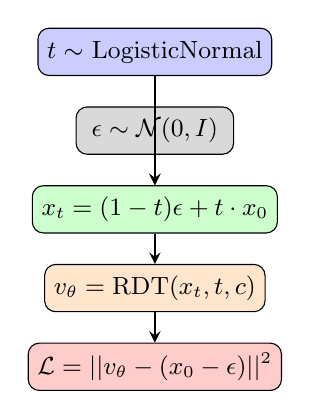
\begin{tikzpicture}[
                block/.style={draw, rounded corners, minimum width=2cm, minimum height=0.6cm, align=center, font=\small},
                arrow/.style={->, thick, >=stealth}
            ]
                % Sample timestep
                \node[block, fill=blue!20] (t) at (0, 4) {$t \sim$ LogisticNormal};

                % Noise
                \node[block, fill=gray!30] (noise) at (0, 3) {$\epsilon \sim \mathcal{N}(0, I)$};

                % Interpolate
                \node[block, fill=green!20] (interp) at (0, 2) {$x_t = (1-t)\epsilon + t \cdot x_0$};

                % Predict
                \node[block, fill=orange!20] (pred) at (0, 1) {$v_\theta = \text{RDT}(x_t, t, c)$};

                % Loss
                \node[block, fill=red!20] (loss) at (0, 0) {$\mathcal{L} = ||v_\theta - (x_0 - \epsilon)||^2$};

                \draw[arrow] (t) -- (interp);
                \draw[arrow] (noise) -- (interp);
                \draw[arrow] (interp) -- (pred);
                \draw[arrow] (pred) -- (loss);
            \end{tikzpicture}
        \end{column}
        \begin{column}{0.5\textwidth}
            \textbf{Inference (5 steps):}
            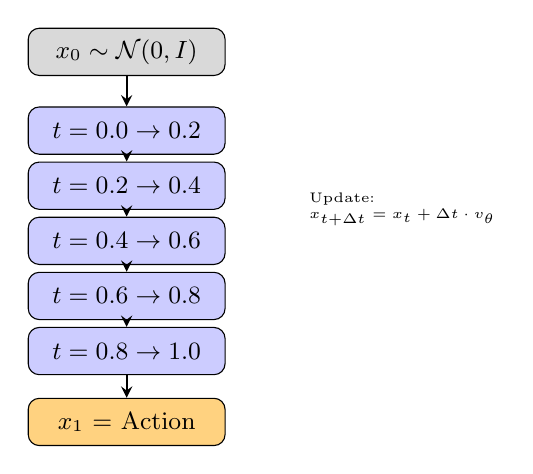
\begin{tikzpicture}[
                block/.style={draw, rounded corners, minimum width=2.5cm, minimum height=0.6cm, align=center, font=\small},
                arrow/.style={->, thick, >=stealth}
            ]
                % Start
                \node[block, fill=gray!30] (x0) at (0, 4) {$x_0 \sim \mathcal{N}(0, I)$};

                % Steps
                \node[block, fill=blue!20] (s1) at (0, 3) {$t=0.0 \rightarrow 0.2$};
                \node[block, fill=blue!20] (s2) at (0, 2.3) {$t=0.2 \rightarrow 0.4$};
                \node[block, fill=blue!20] (s3) at (0, 1.6) {$t=0.4 \rightarrow 0.6$};
                \node[block, fill=blue!20] (s4) at (0, 0.9) {$t=0.6 \rightarrow 0.8$};
                \node[block, fill=blue!20] (s5) at (0, 0.2) {$t=0.8 \rightarrow 1.0$};

                % Output
                \node[block, fill=actionorange!50] (out) at (0, -0.7) {$x_1$ = Action};

                \draw[arrow] (x0) -- (s1);
                \draw[arrow] (s1) -- (s2);
                \draw[arrow] (s2) -- (s3);
                \draw[arrow] (s3) -- (s4);
                \draw[arrow] (s4) -- (s5);
                \draw[arrow] (s5) -- (out);

                % Update formula
                \node[font=\tiny, align=left] at (3.5, 2) {
                    Update:\\
                    $x_{t+\Delta t} = x_t + \Delta t \cdot v_\theta$
                };
            \end{tikzpicture}
        \end{column}
    \end{columns}
\end{frame}

\begin{frame}[fragile]{RDT Inferencer: step() Method}
\begin{lstlisting}[language=Python, title=models/rdt\_inferencer.py: step()]
def step(self, observations, instruction):
    # 1. Extract images by camera_names order
    images = [observations['images'][name] for name in self.camera_names]
    # camera_names: ["left_stereo", "right_stereo"]

    # 2. Convert state to tensor
    state = torch.tensor(observations['state']).reshape(1, 1, -1)
    # Shape: [1, 1, state_dim]

    # 3. Encode images and instruction (with caching)
    if instruction not in self.lang_embeds_cache:
        vlang_kv_cache, vlang_attn_mask = self.encode_image_and_instruction(
            images, instruction
        )
        self.lang_embeds_cache[instruction] = (vlang_kv_cache, vlang_attn_mask)

    # 4. Predict action with RDT policy (5 denoising steps)
    action = self.policy.predict_action(
        states=state,
        img_cond=vlang_kv_cache,
        img_attn_mask=vlang_attn_mask
    )  # Shape: [1, 24, 20]

    # 5. Unnormalize
    action = self.normalizer["action"].unnormalize(action)

    return action.squeeze(0)  # [24, 20]
\end{lstlisting}
\end{frame}

%==============================================================================
\section{Training Pipeline}
%==============================================================================

\begin{frame}{Training Pipeline Overview}
    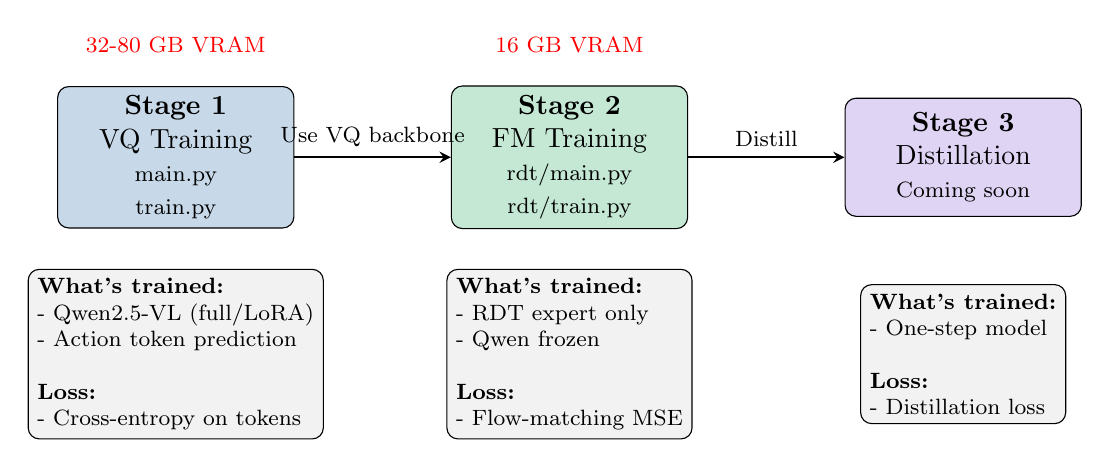
\begin{tikzpicture}[
        stage/.style={draw, rounded corners, fill=blue!20, minimum width=3cm, minimum height=1.5cm, align=center},
        arrow/.style={->, thick, >=stealth}
    ]
        % Stage 1
        \node[stage, fill=qwenblue!30] (s1) at (0, 0) {
            \textbf{Stage 1}\\
            VQ Training\\
            {\footnotesize main.py}\\
            {\footnotesize train.py}
        };

        % Stage 2
        \node[stage, fill=rdtgreen!30] (s2) at (5, 0) {
            \textbf{Stage 2}\\
            FM Training\\
            {\footnotesize rdt/main.py}\\
            {\footnotesize rdt/train.py}
        };

        % Stage 3
        \node[stage, fill=vqpurple!30] (s3) at (10, 0) {
            \textbf{Stage 3}\\
            Distillation\\
            {\footnotesize Coming soon}
        };

        % Details
        \node[draw, rounded corners, fill=gray!10, align=left, font=\footnotesize] (d1) at (0, -2.5) {
            \textbf{What's trained:}\\
            - Qwen2.5-VL (full/LoRA)\\
            - Action token prediction\\
            \\
            \textbf{Loss:}\\
            - Cross-entropy on tokens
        };

        \node[draw, rounded corners, fill=gray!10, align=left, font=\footnotesize] (d2) at (5, -2.5) {
            \textbf{What's trained:}\\
            - RDT expert only\\
            - Qwen frozen\\
            \\
            \textbf{Loss:}\\
            - Flow-matching MSE
        };

        \node[draw, rounded corners, fill=gray!10, align=left, font=\footnotesize] (d3) at (10, -2.5) {
            \textbf{What's trained:}\\
            - One-step model\\
            \\
            \textbf{Loss:}\\
            - Distillation loss
        };

        % Arrows
        \draw[arrow] (s1) -- (s2) node[midway, above, font=\footnotesize] {Use VQ backbone};
        \draw[arrow] (s2) -- (s3) node[midway, above, font=\footnotesize] {Distill};

        % VRAM requirements
        \node[above=0.3cm of s1, font=\footnotesize, text=red] {32-80 GB VRAM};
        \node[above=0.3cm of s2, font=\footnotesize, text=red] {16 GB VRAM};
    \end{tikzpicture}
\end{frame}

\begin{frame}{Stage 1: VLA Training (train.py)}
    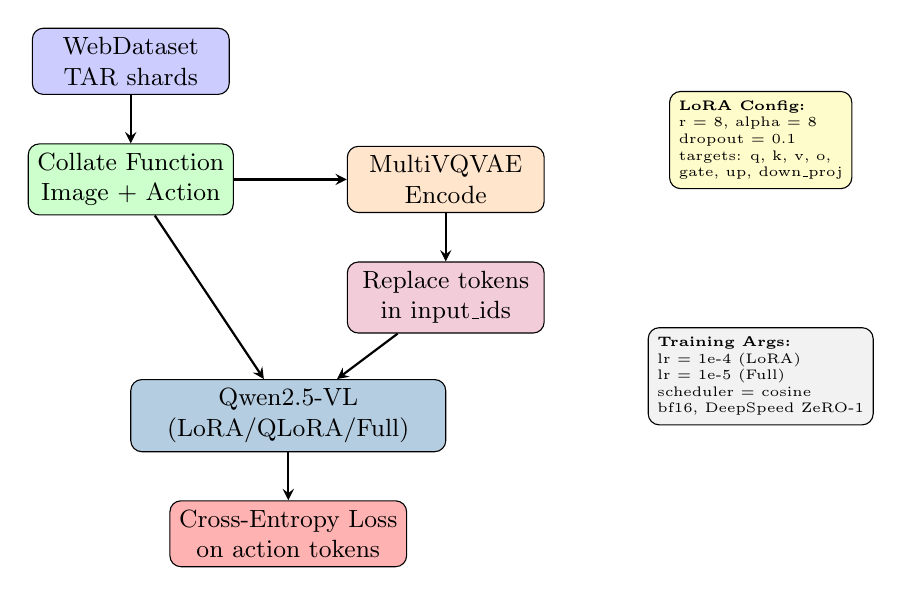
\begin{tikzpicture}[
        block/.style={draw, rounded corners, minimum width=2.5cm, minimum height=0.8cm, align=center, font=\small},
        arrow/.style={->, thick, >=stealth}
    ]
        % Data loading
        \node[block, fill=blue!20] (data) at (0, 3) {WebDataset\\TAR shards};

        % Preprocessing
        \node[block, fill=green!20] (prep) at (0, 1.5) {Collate Function\\Image + Action};

        % Action tokenization
        \node[block, fill=orange!20] (vae) at (4, 1.5) {MultiVQVAE\\Encode};

        % Token embedding
        \node[block, fill=purple!20] (emb) at (4, 0) {Replace tokens\\in input\_ids};

        % Model
        \node[block, fill=qwenblue!40, minimum width=4cm] (model) at (2, -1.5) {
            Qwen2.5-VL\\
            (LoRA/QLoRA/Full)
        };

        % Loss
        \node[block, fill=red!30] (loss) at (2, -3) {
            Cross-Entropy Loss\\
            on action tokens
        };

        % Arrows
        \draw[arrow] (data) -- (prep);
        \draw[arrow] (prep) -- (vae);
        \draw[arrow] (vae) -- (emb);
        \draw[arrow] (prep) -- (model);
        \draw[arrow] (emb) -- (model);
        \draw[arrow] (model) -- (loss);

        % LoRA config
        \node[draw, rounded corners, fill=yellow!20, align=left, font=\tiny] at (8, 2) {
            \textbf{LoRA Config:}\\
            r = 8, alpha = 8\\
            dropout = 0.1\\
            targets: q, k, v, o,\\
            gate, up, down\_proj
        };

        % Training args
        \node[draw, rounded corners, fill=gray!10, align=left, font=\tiny] at (8, -1) {
            \textbf{Training Args:}\\
            lr = 1e-4 (LoRA)\\
            lr = 1e-5 (Full)\\
            scheduler = cosine\\
            bf16, DeepSpeed ZeRO-1
        };
    \end{tikzpicture}
\end{frame}

\begin{frame}{Stage 2: RDT Training (rdt/train.py)}
    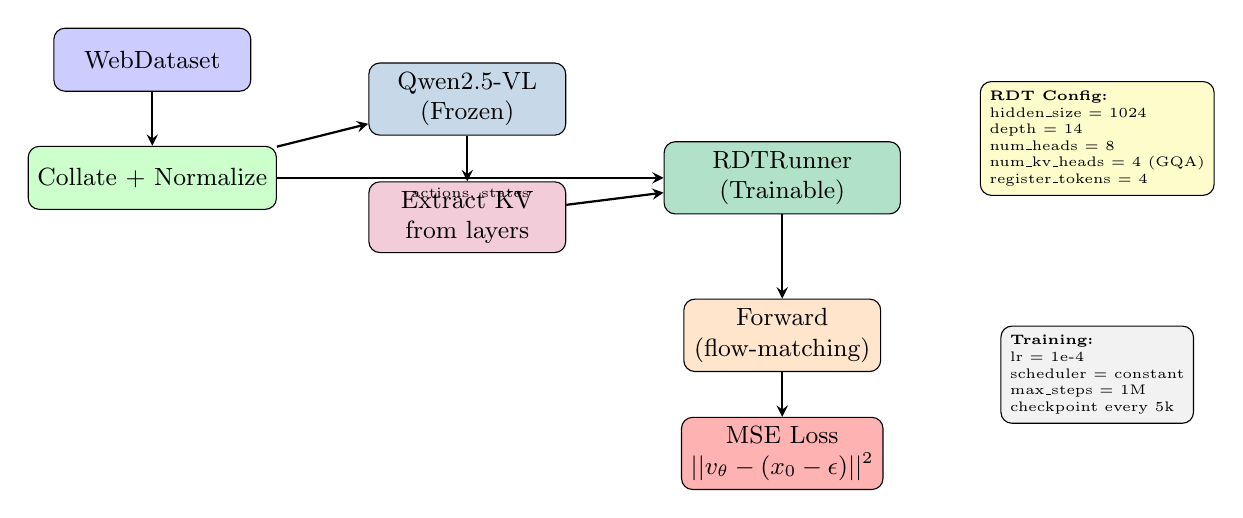
\begin{tikzpicture}[
        block/.style={draw, rounded corners, minimum width=2.5cm, minimum height=0.8cm, align=center, font=\small},
        arrow/.style={->, thick, >=stealth}
    ]
        % Data
        \node[block, fill=blue!20] (data) at (0, 3) {WebDataset};

        % Collate
        \node[block, fill=green!20] (coll) at (0, 1.5) {Collate + Normalize};

        % Qwen (frozen)
        \node[block, fill=qwenblue!30] (qwen) at (4, 2.5) {Qwen2.5-VL\\(Frozen)};

        % KV extraction
        \node[block, fill=purple!20] (kv) at (4, 1) {Extract KV\\from layers};

        % RDT
        \node[block, fill=rdtgreen!40, minimum width=3cm] (rdt) at (8, 1.5) {RDTRunner\\(Trainable)};

        % Forward
        \node[block, fill=orange!20] (fwd) at (8, -0.5) {
            Forward\\
            (flow-matching)
        };

        % Loss
        \node[block, fill=red!30] (loss) at (8, -2) {
            MSE Loss\\
            $||v_\theta - (x_0 - \epsilon)||^2$
        };

        % Arrows
        \draw[arrow] (data) -- (coll);
        \draw[arrow] (coll) -- (qwen);
        \draw[arrow] (qwen) -- (kv);
        \draw[arrow] (kv) -- (rdt);
        \draw[arrow] (coll) -- (rdt) node[midway, below, font=\tiny] {actions, states};
        \draw[arrow] (rdt) -- (fwd);
        \draw[arrow] (fwd) -- (loss);

        % Config
        \node[draw, rounded corners, fill=yellow!20, align=left, font=\tiny] at (12, 2) {
            \textbf{RDT Config:}\\
            hidden\_size = 1024\\
            depth = 14\\
            num\_heads = 8\\
            num\_kv\_heads = 4 (GQA)\\
            register\_tokens = 4
        };

        % Training
        \node[draw, rounded corners, fill=gray!10, align=left, font=\tiny] at (12, -1) {
            \textbf{Training:}\\
            lr = 1e-4\\
            scheduler = constant\\
            max\_steps = 1M\\
            checkpoint every 5k
        };
    \end{tikzpicture}
\end{frame}

%==============================================================================
\section{Inference Pipeline}
%==============================================================================

\begin{frame}{Complete Inference Pipeline: RDT2-VQ}
    \begin{tikzpicture}[
        block/.style={draw, rounded corners, minimum width=2cm, minimum height=0.6cm, align=center, font=\tiny},
        arrow/.style={->, thick, >=stealth}
    ]
        % Scale
        \def\yscale{0.9}

        % Camera input
        \node[block, fill=blue!20] (cam1) at (0, 5*\yscale) {Left Camera\\384$\times$384};
        \node[block, fill=blue!20] (cam2) at (2.5, 5*\yscale) {Right Camera\\384$\times$384};

        % Concatenate
        \node[block, fill=green!20] (concat) at (1.25, 3.5*\yscale) {Concatenate\\384$\times$768};

        % JPEG (optional)
        \node[block, fill=orange!20] (jpeg) at (1.25, 2.5*\yscale) {JPEG Compress\\(if trained with)};

        % Instruction
        \node[block, fill=yellow!20] (instr) at (4.5, 3.5*\yscale) {Instruction\\"Pick up..."};

        % Chat template
        \node[block, fill=gray!20, minimum width=3cm] (chat) at (3, 1.5*\yscale) {Chat Template\\+ Guidance tokens};

        % Processor
        \node[block, fill=purple!20] (proc) at (3, 0.5*\yscale) {Qwen Processor\\Tokenize};

        % Model
        \node[block, fill=qwenblue!40, minimum width=3cm] (model) at (3, -0.7*\yscale) {Qwen2.5-VL\\Generate (27 tokens)};

        % Extract
        \node[block, fill=red!20] (extract) at (7, -0.7*\yscale) {Extract Action IDs\\between markers};

        % Convert
        \node[block, fill=orange!30] (convert) at (7, -2*\yscale) {vocab - (id + 1)\\Clamp [0, 1023]};

        % VAE decode
        \node[block, fill=vqpurple!40] (vae) at (7, -3.2*\yscale) {MultiVQVAE\\Decode};

        % Unnormalize
        \node[block, fill=green!30] (unnorm) at (7, -4.4*\yscale) {Unnormalize\\LinearNormalizer};

        % Gripper scale
        \node[block, fill=yellow!30] (grip) at (11, -3.2*\yscale) {Gripper Rescale\\/ 0.088 * 0.10};

        % Output
        \node[block, fill=actionorange!50, minimum width=2.5cm] (out) at (11, -4.4*\yscale) {Action Chunk\\[24, 20]};

        % Robot
        \node[block, fill=datared!30] (robot) at (11, -5.5*\yscale) {Execute on Robot};

        % Arrows
        \draw[arrow] (cam1) -- (concat);
        \draw[arrow] (cam2) -- (concat);
        \draw[arrow] (concat) -- (jpeg);
        \draw[arrow] (jpeg) -- (chat);
        \draw[arrow] (instr) -- (chat);
        \draw[arrow] (chat) -- (proc);
        \draw[arrow] (proc) -- (model);
        \draw[arrow] (model) -- (extract);
        \draw[arrow] (extract) -- (convert);
        \draw[arrow] (convert) -- (vae);
        \draw[arrow] (vae) -- (unnorm);
        \draw[arrow] (unnorm) -- (grip);
        \draw[arrow] (grip) -- (out);
        \draw[arrow] (out) -- (robot);
    \end{tikzpicture}
\end{frame}

\begin{frame}{Complete Inference Pipeline: RDT2-FM}
    \begin{tikzpicture}[
        block/.style={draw, rounded corners, minimum width=2cm, minimum height=0.6cm, align=center, font=\tiny},
        arrow/.style={->, thick, >=stealth}
    ]
        % Scale
        \def\yscale{0.9}

        % Camera input
        \node[block, fill=blue!20] (cam1) at (0, 5*\yscale) {Left Camera\\384$\times$384};
        \node[block, fill=blue!20] (cam2) at (2.5, 5*\yscale) {Right Camera\\384$\times$384};

        % Concatenate
        \node[block, fill=green!20] (concat) at (1.25, 3.5*\yscale) {Concatenate\\384$\times$768};

        % Instruction
        \node[block, fill=yellow!20] (instr) at (4.5, 3.5*\yscale) {Instruction};

        % State
        \node[block, fill=orange!20] (state) at (7, 3.5*\yscale) {State\\[1, 1, 20]};

        % Preprocess
        \node[block, fill=purple!20, minimum width=3cm] (prep) at (3, 2*\yscale) {prepare\_data\_from\_vlm\\Chat template};

        % Qwen (frozen)
        \node[block, fill=qwenblue!30, minimum width=3cm] (qwen) at (3, 0.5*\yscale) {Qwen2.5-VL (Frozen)\\Extract KV Cache};

        % Cache
        \node[block, fill=gray!20] (cache) at (3, -0.8*\yscale) {vlang\_kv\_cache\\vlang\_attn\_mask};

        % RDT
        \node[block, fill=rdtgreen!50, minimum width=3cm] (rdt) at (7, 0*\yscale) {RDT Action Expert\\predict\_action()};

        % Noise
        \node[block, fill=gray!30] (noise) at (10, 1.5*\yscale) {Noise\\$\mathcal{N}(0, I)$};

        % Denoise
        \node[block, fill=blue!30] (denoise) at (7, -1.5*\yscale) {5 Denoising Steps};

        % Unnormalize
        \node[block, fill=green!30] (unnorm) at (7, -3*\yscale) {Unnormalize\\LinearNormalizer};

        % Gripper
        \node[block, fill=yellow!30] (grip) at (11, -1.5*\yscale) {Gripper Rescale\\/ 0.088 * 0.10};

        % Output
        \node[block, fill=actionorange!50, minimum width=2.5cm] (out) at (11, -3*\yscale) {Action Chunk\\[24, 20]};

        % Robot
        \node[block, fill=datared!30] (robot) at (11, -4.2*\yscale) {Execute on Robot};

        % Arrows
        \draw[arrow] (cam1) -- (concat);
        \draw[arrow] (cam2) -- (concat);
        \draw[arrow] (concat) -- (prep);
        \draw[arrow] (instr) -- (prep);
        \draw[arrow] (prep) -- (qwen);
        \draw[arrow] (qwen) -- (cache);
        \draw[arrow] (cache) -- (rdt);
        \draw[arrow] (state) -- (rdt);
        \draw[arrow] (noise) -- (rdt);
        \draw[arrow] (rdt) -- (denoise);
        \draw[arrow] (denoise) -- (unnorm);
        \draw[arrow] (unnorm) -- (grip);
        \draw[arrow] (grip) -- (out);
        \draw[arrow] (out) -- (robot);
    \end{tikzpicture}
\end{frame}

%==============================================================================
\section{Normalizer}
%==============================================================================

\begin{frame}{LinearNormalizer: Importance for Inference}
    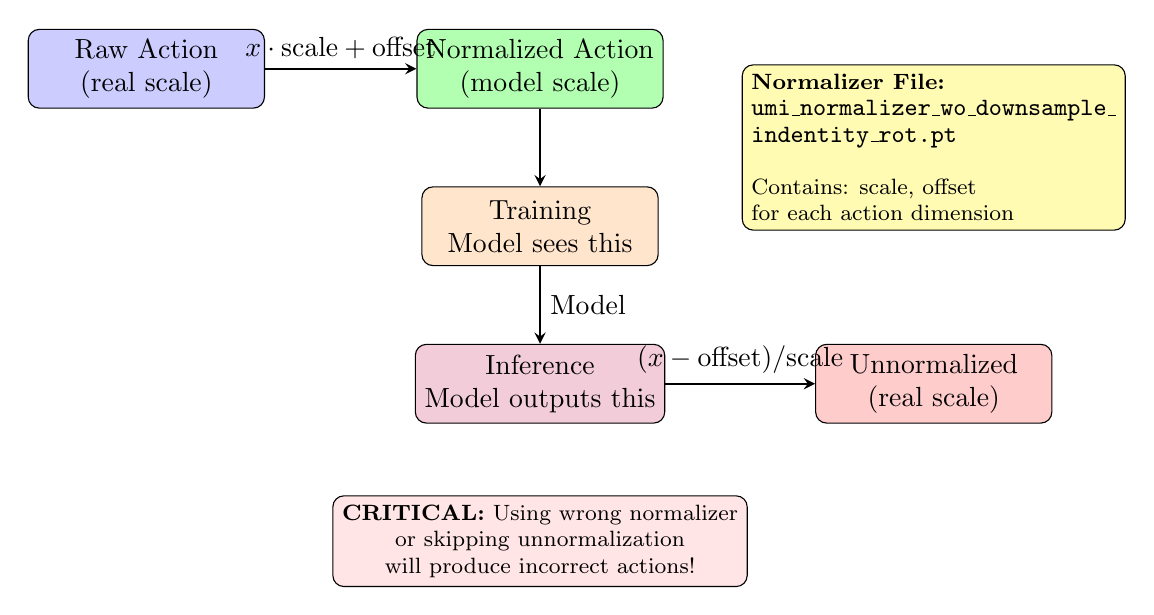
\begin{tikzpicture}[
        block/.style={draw, rounded corners, minimum width=3cm, minimum height=1cm, align=center},
        arrow/.style={->, thick, >=stealth}
    ]
        % Raw action
        \node[block, fill=blue!20] (raw) at (0, 2) {Raw Action\\(real scale)};

        % Normalize
        \node[block, fill=green!30] (norm) at (5, 2) {Normalized Action\\(model scale)};

        % Training
        \node[block, fill=orange!20] (train) at (5, 0) {Training\\Model sees this};

        % Inference
        \node[block, fill=purple!20] (inf) at (5, -2) {Inference\\Model outputs this};

        % Unnormalize
        \node[block, fill=red!20] (unnorm) at (10, -2) {Unnormalized\\(real scale)};

        % Arrows
        \draw[arrow] (raw) -- (norm) node[midway, above] {$x \cdot \text{scale} + \text{offset}$};
        \draw[arrow] (norm) -- (train);
        \draw[arrow] (train) -- (inf) node[midway, right] {Model};
        \draw[arrow] (inf) -- (unnorm) node[midway, above] {$(x - \text{offset}) / \text{scale}$};

        % Normalizer file
        \node[draw, rounded corners, fill=yellow!30, align=left, font=\footnotesize] at (10, 1) {
            \textbf{Normalizer File:}\\
            \code{umi\_normalizer\_wo\_downsample\_}\\
            \code{indentity\_rot.pt}\\
            \\
            Contains: scale, offset\\
            for each action dimension
        };

        % Warning
        \node[draw, rounded corners, fill=red!10, align=center, font=\footnotesize] at (5, -4) {
            \textbf{CRITICAL:} Using wrong normalizer\\
            or skipping unnormalization\\
            will produce incorrect actions!
        };
    \end{tikzpicture}
\end{frame}

\begin{frame}{Normalizer: Implementation Details}
    \begin{columns}
        \begin{column}{0.5\textwidth}
            \textbf{LinearNormalizer Class:}
            \begin{itemize}
                \item Supports multiple fields: \code{action}, \code{state}
                \item Modes: \code{limits} (min-max), \code{gaussian} (standardization)
                \item Per-dimension scale and offset
            \end{itemize}

            \vspace{0.3cm}
            \textbf{Key Methods:}
            \begin{itemize}
                \item \code{normalize(x)}: Forward transform
                \item \code{unnormalize(x)}: Inverse transform
                \item \code{load(filepath)}: Load from checkpoint
                \item \code{["action"]}: Field accessor
            \end{itemize}
        \end{column}
        \begin{column}{0.5\textwidth}
            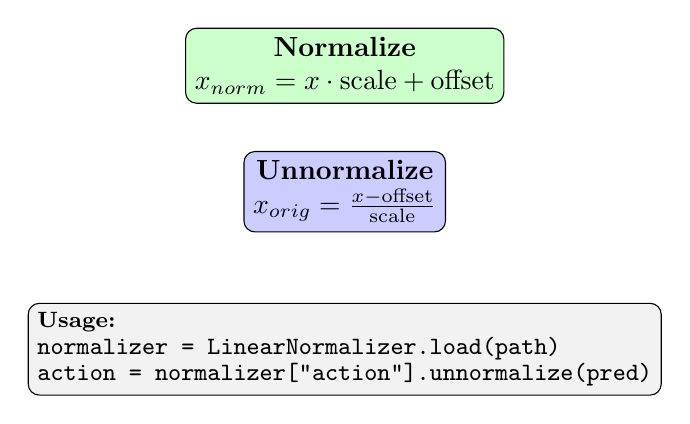
\begin{tikzpicture}[scale=0.8]
                % Normalize formula
                \node[draw, rounded corners, fill=green!20, align=center] (norm) at (0, 3) {
                    \textbf{Normalize}\\
                    $x_{norm} = x \cdot \text{scale} + \text{offset}$
                };

                % Unnormalize formula
                \node[draw, rounded corners, fill=blue!20, align=center] (unnorm) at (0, 1) {
                    \textbf{Unnormalize}\\
                    $x_{orig} = \frac{x - \text{offset}}{\text{scale}}$
                };

                % Usage
                \node[draw, rounded corners, fill=gray!10, align=left, font=\footnotesize] (use) at (0, -1.5) {
                    \textbf{Usage:}\\
                    \code{normalizer = LinearNormalizer.load(path)}\\
                    \code{action = normalizer["action"].unnormalize(pred)}
                };
            \end{tikzpicture}
        \end{column}
    \end{columns}
\end{frame}

%==============================================================================
\section{ManiSkill Integration}
%==============================================================================

\begin{frame}{ManiSkill Integration: Key Considerations}
    \begin{tikzpicture}[
        issue/.style={draw, rounded corners, fill=red!20, minimum width=4cm, minimum height=1cm, align=center},
        solution/.style={draw, rounded corners, fill=green!20, minimum width=4cm, minimum height=1cm, align=center}
    ]
        % Issues column
        \node[font=\large\bfseries] at (2, 5) {Potential Issues};

        \node[issue] (i1) at (2, 3.5) {Wrong camera order\\Left/Right swapped};
        \node[issue] (i2) at (2, 2) {Image resolution\\mismatch};
        \node[issue] (i3) at (2, 0.5) {Missing normalizer\\or wrong path};
        \node[issue] (i4) at (2, -1) {Action space\\mismatch};
        \node[issue] (i5) at (2, -2.5) {Gripper scale\\not applied};

        % Solutions column
        \node[font=\large\bfseries] at (10, 5) {Solutions};

        \node[solution] (s1) at (10, 3.5) {Check camera\_names order\\["left\_stereo", "right\_stereo"]};
        \node[solution] (s2) at (10, 2) {Resize to 384$\times$384\\per camera};
        \node[solution] (s3) at (10, 0.5) {Load correct normalizer\\for UMI data};
        \node[solution] (s4) at (10, -1) {Verify 20D bimanual\\or 10D single arm};
        \node[solution] (s5) at (10, -2.5) {Apply: action / 0.088 * 0.10};

        % Arrows
        \draw[->, thick] (i1) -- (s1);
        \draw[->, thick] (i2) -- (s2);
        \draw[->, thick] (i3) -- (s3);
        \draw[->, thick] (i4) -- (s4);
        \draw[->, thick] (i5) -- (s5);
    \end{tikzpicture}
\end{frame}

\begin{frame}{Debugging Checklist: Franka + Wrist Camera}
    \begin{columns}
        \begin{column}{0.5\textwidth}
            \textbf{Image Input:}
            \begin{itemize}
                \item[$\square$] Resolution: 384 $\times$ 384 per camera
                \item[$\square$] Format: RGB, uint8
                \item[$\square$] Concatenation: Left | Right = 384 $\times$ 768
                \item[$\square$] JPEG compression if model trained with it
            \end{itemize}

            \vspace{0.3cm}
            \textbf{Instruction:}
            \begin{itemize}
                \item[$\square$] Format: "Verb + Object."
                \item[$\square$] Capitalized first letter
                \item[$\square$] Period at end
            \end{itemize}
        \end{column}
        \begin{column}{0.5\textwidth}
            \textbf{Action Output:}
            \begin{itemize}
                \item[$\square$] Shape: (24, 20) or (24, 10)
                \item[$\square$] Unnormalized with correct normalizer
                \item[$\square$] Gripper rescaled: / 0.088 * 0.10
                \item[$\square$] Position in meters
                \item[$\square$] Rotation in 6D representation
            \end{itemize}

            \vspace{0.3cm}
            \textbf{State Input (FM only):}
            \begin{itemize}
                \item[$\square$] Shape: (state\_dim,)
                \item[$\square$] Can be zeros for inference
            \end{itemize}
        \end{column}
    \end{columns}

    \vspace{0.5cm}
    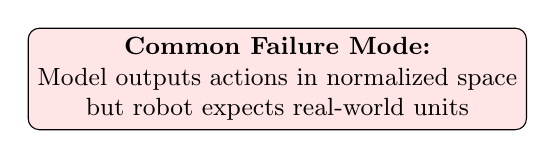
\begin{tikzpicture}
        \node[draw, rounded corners, fill=red!10, align=center, font=\small] at (6, 0) {
            \textbf{Common Failure Mode:}\\
            Model outputs actions in normalized space\\
            but robot expects real-world units
        };
    \end{tikzpicture}
\end{frame}

\begin{frame}{Single Arm Adaptation}
    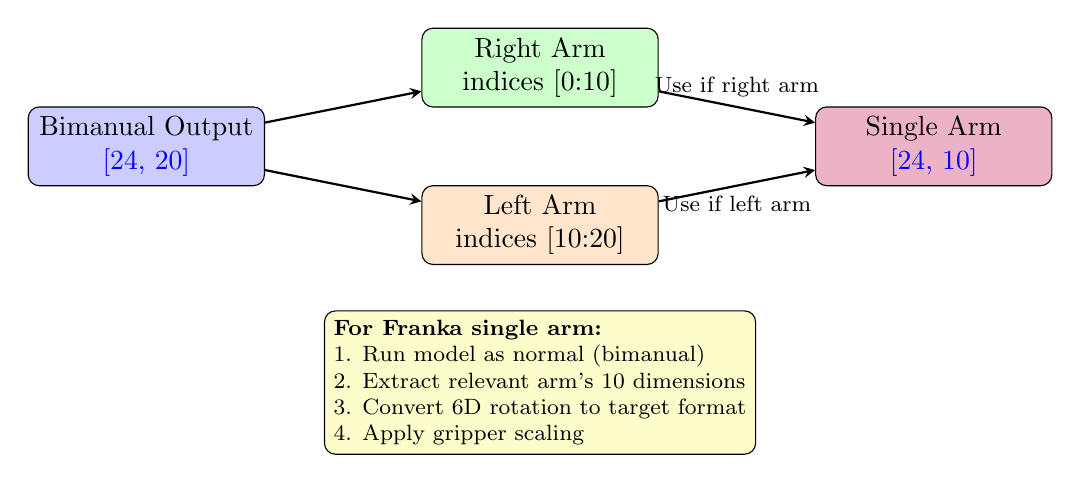
\begin{tikzpicture}[
        block/.style={draw, rounded corners, minimum width=3cm, minimum height=1cm, align=center},
        arrow/.style={->, thick, >=stealth}
    ]
        % Original
        \node[block, fill=blue!20] (orig) at (0, 2) {
            Bimanual Output\\
            \dimension{24, 20}
        };

        % Right arm
        \node[block, fill=green!20] (right) at (5, 3) {
            Right Arm\\
            indices [0:10]
        };

        % Left arm
        \node[block, fill=orange!20] (left) at (5, 1) {
            Left Arm\\
            indices [10:20]
        };

        % Single arm
        \node[block, fill=purple!30] (single) at (10, 2) {
            Single Arm\\
            \dimension{24, 10}
        };

        % Arrows
        \draw[arrow] (orig) -- (right);
        \draw[arrow] (orig) -- (left);
        \draw[arrow] (right) -- (single) node[midway, above, font=\footnotesize] {Use if right arm};
        \draw[arrow] (left) -- (single) node[midway, below, font=\footnotesize] {Use if left arm};

        % Note
        \node[draw, rounded corners, fill=yellow!20, align=left, font=\footnotesize] at (5, -1) {
            \textbf{For Franka single arm:}\\
            1. Run model as normal (bimanual)\\
            2. Extract relevant arm's 10 dimensions\\
            3. Convert 6D rotation to target format\\
            4. Apply gripper scaling
        };
    \end{tikzpicture}
\end{frame}

\begin{frame}{6D Rotation to Axis-Angle Conversion}
    \begin{columns}
        \begin{column}{0.5\textwidth}
            \textbf{RDT2 outputs 6D rotation}

            \vspace{0.3cm}
            \textbf{Franka may need:}
            \begin{itemize}
                \item Quaternion (w, x, y, z)
                \item Axis-angle (rx, ry, rz)
                \item Rotation matrix (3$\times$3)
            \end{itemize}

            \vspace{0.3cm}
            \textbf{Conversion Pipeline:}
            \begin{enumerate}
                \item 6D $\rightarrow$ 3$\times$3 matrix
                \item 3$\times$3 $\rightarrow$ target format
            \end{enumerate}
        \end{column}
        \begin{column}{0.5\textwidth}
            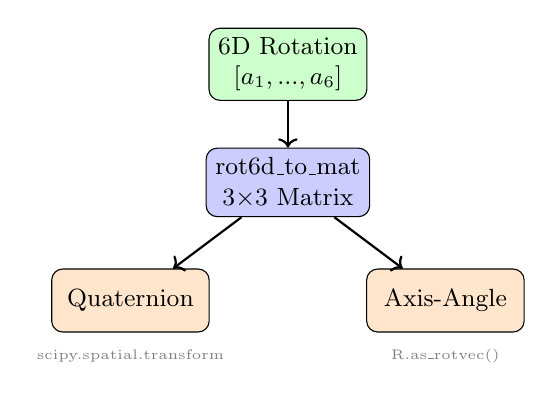
\begin{tikzpicture}[
                block/.style={draw, rounded corners, minimum width=2cm, minimum height=0.8cm, align=center, font=\small}
            ]
                \node[block, fill=green!20] (r6d) at (0, 3) {6D Rotation\\$[a_1, ..., a_6]$};

                \node[block, fill=blue!20] (mat) at (0, 1.5) {rot6d\_to\_mat\\3$\times$3 Matrix};

                \node[block, fill=orange!20] (quat) at (-2, 0) {Quaternion};
                \node[block, fill=orange!20] (axis) at (2, 0) {Axis-Angle};

                \draw[->, thick] (r6d) -- (mat);
                \draw[->, thick] (mat) -- (quat);
                \draw[->, thick] (mat) -- (axis);

                % Functions
                \node[font=\tiny, text=gray] at (-2, -0.7) {scipy.spatial.transform};
                \node[font=\tiny, text=gray] at (2, -0.7) {R.as\_rotvec()};
            \end{tikzpicture}
        \end{column}
    \end{columns}
\end{frame}

%==============================================================================
\section{File Reference}
%==============================================================================

\begin{frame}{Key Files: Training}
    \begin{tabular}{p{5cm}p{8cm}}
        \toprule
        \textbf{File} & \textbf{Purpose} \\
        \midrule
        \code{main.py} & VLA training entry point \\
        \code{train.py} & VLA training loop \\
        \code{rdt/main.py} & RDT expert training entry \\
        \code{rdt/train.py} & RDT training loop \\
        \code{vla\_trainer.py} & Custom HF Trainer \\
        \code{rdt/dataset.py} & WebDataset loading \\
        \code{data/umi\_video\_dataset.py} & UMI video dataset \\
        \code{scripts/finetune\_lora.sh} & LoRA fine-tuning script \\
        \code{scripts/finetune\_rdt.sh} & RDT fine-tuning script \\
        \code{scripts/zero1.json} & DeepSpeed config \\
        \bottomrule
    \end{tabular}
\end{frame}

\begin{frame}{Key Files: Inference}
    \begin{tabular}{p{6cm}p{7cm}}
        \toprule
        \textbf{File} & \textbf{Purpose} \\
        \midrule
        \code{deploy/inference\_real\_vq.py} & RDT2-VQ inference \\
        \code{deploy/inference\_real\_fm.py} & RDT2-FM inference \\
        \code{models/rdt\_inferencer.py} & High-level inference wrapper \\
        \code{utils.py} & batch\_predict\_action() \\
        \code{deploy/vllm\_utils.py} & vLLM accelerated inference \\
        \code{models/normalizer/normalizer.py} & LinearNormalizer \\
        \bottomrule
    \end{tabular}
\end{frame}

\begin{frame}{Key Files: Model Architecture}
    \begin{tabular}{p{5.5cm}p{7.5cm}}
        \toprule
        \textbf{File} & \textbf{Purpose} \\
        \midrule
        \code{models/rdt\_runner.py} & RDT diffusion wrapper \\
        \code{models/rdt/model.py} & RDT transformer architecture \\
        \code{models/rdt/blocks.py} & Transformer building blocks \\
        \code{vqvae/models/vq.py} & Vector Quantizer \\
        \code{vqvae/models/rvq.py} & Residual VQ \\
        \code{vqvae/models/vqvae.py} & VQ-VAE autoencoder \\
        \code{vqvae/models/multivqvae.py} & Multi-component VQVAE \\
        \code{vqvae/models/cnn/model.py} & CNN encoder/decoder \\
        \bottomrule
    \end{tabular}
\end{frame}

\begin{frame}{Key Files: Configuration}
    \begin{tabular}{p{6cm}p{7cm}}
        \toprule
        \textbf{File} & \textbf{Purpose} \\
        \midrule
        \code{configs/rdt/post\_train.yaml} & RDT model config \\
        \code{configs/datasets/example.yaml} & Dataset template \\
        \code{configs/robots/eval\_bimanual\_*.yaml} & Robot hardware config \\
        \bottomrule
    \end{tabular}

    \vspace{0.5cm}
    \textbf{Important Config Values:}
    \begin{itemize}
        \item \code{action\_chunk\_size}: 24
        \item \code{action\_dim}: 20 (bimanual)
        \item \code{state\_dim}: 20
        \item \code{num\_cameras}: 2
        \item \code{hidden\_size}: 1024
        \item \code{depth}: 14
        \item \code{num\_inference\_timesteps}: 5
    \end{itemize}
\end{frame}

%==============================================================================
\section{Summary}
%==============================================================================

\begin{frame}{Summary: Complete Data Flow}
    \begin{tikzpicture}[
        block/.style={draw, rounded corners, minimum width=2cm, minimum height=0.6cm, align=center, font=\tiny},
        arrow/.style={->, thick, >=stealth}
    ]
        % Input
        \node[block, fill=blue!20] (img) at (0, 3) {2$\times$Camera\\384$\times$384};
        \node[block, fill=green!20] (instr) at (0, 2) {Instruction};

        % Processing
        \node[block, fill=orange!20] (concat) at (3, 2.5) {Concat\\384$\times$768};

        % Model choice
        \node[block, fill=qwenblue!30, minimum width=2.5cm] (vq) at (6, 3.5) {RDT2-VQ\\27 tokens};
        \node[block, fill=rdtgreen!40, minimum width=2.5cm] (fm) at (6, 1.5) {RDT2-FM\\5 denoise};

        % Decode
        \node[block, fill=vqpurple!30] (vae) at (9, 3.5) {VQVAE\\Decode};

        % Merge
        \node[block, fill=yellow!30] (action) at (11, 2.5) {Action\\[24, 20]};

        % Post-process
        \node[block, fill=red!20] (unnorm) at (11, 1) {Unnormalize\\+ Gripper scale};

        % Robot
        \node[block, fill=datared!40] (robot) at (11, -0.5) {Robot\\Execution};

        % Arrows
        \draw[arrow] (img) -- (concat);
        \draw[arrow] (instr) -- (concat);
        \draw[arrow] (concat) -- (vq);
        \draw[arrow] (concat) -- (fm);
        \draw[arrow] (vq) -- (vae);
        \draw[arrow] (vae) -- (action);
        \draw[arrow] (fm) -- (action);
        \draw[arrow] (action) -- (unnorm);
        \draw[arrow] (unnorm) -- (robot);

        % Dimension annotations
        \node[font=\tiny, text=gray] at (4.5, 3) {[B,C,H,W]};
        \node[font=\tiny, text=gray] at (7.5, 4) {[B,27]};
        \node[font=\tiny, text=gray] at (9.5, 3) {[B,24,20]};
    \end{tikzpicture}

    \vspace{0.5cm}
    \textbf{Key Dimensions to Remember:}
    \begin{itemize}
        \item Image: 384 $\times$ 384 $\times$ 3 per camera
        \item Action tokens: 27 (VQ) or continuous (FM)
        \item Action chunk: 24 timesteps $\times$ 20 dimensions
        \item Per arm: 3 position + 6 rotation + 1 gripper = 10D
    \end{itemize}
\end{frame}

\begin{frame}{Quick Reference Card}
    \begin{columns}
        \begin{column}{0.5\textwidth}
            \textbf{Action Indices:}
            \begin{itemize}
                \item Right pos: [0, 1, 2]
                \item Right rot: [3, 4, 5, 6, 7, 8]
                \item Right grip: [9]
                \item Left pos: [10, 11, 12]
                \item Left rot: [13, 14, 15, 16, 17, 18]
                \item Left grip: [19]
            \end{itemize}

            \vspace{0.3cm}
            \textbf{Token Counts:}
            \begin{itemize}
                \item Position: 18 tokens
                \item Rotation: 9 tokens
                \item Gripper: 3 tokens
                \item Total: 27 tokens
            \end{itemize}
        \end{column}
        \begin{column}{0.5\textwidth}
            \textbf{Critical Operations:}
            \begin{itemize}
                \item Gripper scale: / 0.088 * 0.10
                \item Token convert: vocab - (id + 1)
                \item Clamp: [0, 1023]
            \end{itemize}

            \vspace{0.3cm}
            \textbf{HuggingFace Models:}
            \begin{itemize}
                \item VQ: robotics-diffusion-transformer/RDT2-VQ
                \item FM: robotics-diffusion-transformer/RDT2-FM
                \item VAE: robotics-diffusion-transformer/RVQActionTokenizer
            \end{itemize}
        \end{column}
    \end{columns}
\end{frame}

\begin{frame}{}
    \centering
    \Huge Thank You

    \vspace{1cm}
    \Large Questions?

    \vspace{1cm}
    \normalsize
    \begin{tabular}{ll}
        GitHub: & \url{https://github.com/thu-ml/RDT2} \\
        Project: & \url{https://rdt-robotics.github.io/rdt2/} \\
        Models: & \url{https://huggingface.co/robotics-diffusion-transformer} \\
    \end{tabular}
\end{frame}

\end{document}
